\documentclass[11pt]{article}
\usepackage[T1]{fontenc}
\usepackage[utf8]{inputenc}
\usepackage{lmodern}
\usepackage[margin=1in]{geometry}
\usepackage{amsmath,amssymb,amsthm,mathtools}
\usepackage{booktabs}
\usepackage{array}
\usepackage{graphicx}
\usepackage{microtype}
\usepackage[dvipsnames]{xcolor}
\usepackage[numbers,sort&compress]{natbib}
\usepackage[colorlinks=true,linkcolor=MidnightBlue,citecolor=MidnightBlue,
  urlcolor=MidnightBlue,breaklinks=true]{hyperref}
\hypersetup{pdftitle={A subexponential algorithm for the erasure logical error rate of sparse stabilizer codes},
  pdfauthor={Oliver D'Souza}}
\urlstyle{same}
\setlength{\parskip}{3pt}
\setlength{\emergencystretch}{1.5em}
\newtheorem{theorem}{Theorem}
\newtheorem{corollary}[theorem]{Corollary}
\newtheorem{proposition}[theorem]{Proposition}
\newtheorem{lemma}[theorem]{Lemma}
\theoremstyle{remark}
\newtheorem{remark}[theorem]{Remark}
\newcommand{\F}{\mathbb F_2}
\newcommand{\E}{\mathbb E}
\newcommand{\Prob}{\mathbb P}
\newcommand{\Good}{\mathsf{Good}}
\newcommand{\Bad}{\mathsf{Bad}}
\newcommand{\poly}{\operatorname{poly}}
\newcommand{\rank}{\operatorname{rank}}
\newcommand{\tr}{\operatorname{tr}}
\newcommand{\eps}{\varepsilon}
\newcommand{\pair}[2]{\langle #1,#2\rangle_s}
\newcommand{\Bern}[2]{\binom{#1}{#2}p^{#2}(1-p)^{#1-#2}}
\newcommand{\lean}[1]{\texttt{#1}}
\title{A subexponential algorithm for the erasure logical error rate\\
of sparse stabilizer codes}
\author{Oliver D'Souza\thanks{Copyright \textcopyright\ 2026 Oliver D'Souza.
This paper is licensed under
\href{https://creativecommons.org/licenses/by/4.0/}{Creative Commons Attribution 4.0 International (CC BY 4.0)}.}}
\date{\small 12 November 2026}
\usepackage{longtable}
\begin{document}
\maketitle
\vspace{-1.8em}
\begin{abstract}
How well a quantum error-correcting code protects against the loss of
qubits is measured by the logical error rate \(I_H(p)\) of the optimal
erasure decoder, as a function of the loss probability \(p\). For a
stabilizer code on \(n\) qubits this is an average over all \(2^n\)
erased sets; it is exponentially small at the loss rates of interest,
where simulation sees no failures, and we know of no algorithm faster
than enumeration. We show that the whole curve can be computed to
relative accuracy with a SAT solver, using polynomially many
satisfiability questions about formulas whose size is \emph{linear} in
the size of the code. Precisely, let \(H\) be a sparse check matrix and
\(F_H=1-I_H\) the optimal entanglement fidelity. For any bounded-density
3-SAT algorithm with time \(\poly\cdot T(v)\) and polynomial space, a
randomized algorithm computes, in time
\(\poly(\mathrm{input},\eps^{-1},\log\delta^{-1})\,T(O(n))\) and
polynomial space, a monotone polynomial that approximates \emph{both}
\(I_H\) and \(F_H\) to relative error \(\eps\), simultaneously at every
\(p\in[0,1]\), with probability \(1-\delta\). Two features separate this
from approximate counting with an oracle. The logical error rate is
itself a projected count, through a second certificate complementary to
the one for the fidelity, which gives relative accuracy in the tail that
matters; and every query has \(O(n)\) variables, without which a
subexponential SAT algorithm would yield nothing. With the
machine-checked subexponential 3-SAT algorithm of OpenAI the running
time is \(\poly\cdot2^{O(n(\log\log n)^2/\sqrt{\log n})}\) with polynomial
space, unconditionally, and the reduction, the engine and their
composition are kernel-checked in one Lean~4 development with standard
axioms only. Conversely, any
output meeting the guarantee determines the code distance, and so does a
single value of \(I_H\) at a small explicit \(p\) known up to an
exponential factor; the task is therefore NP-hard already for sparse
codes. The speed-up is asymptotic; for codes of practical size we
combine the same certificate
with sampling and compute logical error rates down to \(10^{-28}\) for
surface, toric and bivariate bicycle codes of up to 128 qubits, with
the distance, the minimum-size failure sets and the leading coefficient
certified by proof-checked SAT refutations. The reduction extends to
correlated erasures generated by linear-size circuits from latent bits
in a fixed number of probability classes. The Lean development, the
code and the data are available at
\url{https://github.com/Oliverds321/stabilizer-erasure-sat-lean}.
\end{abstract}

\section{Introduction}
\label{sec:intro}

A stabilizer code that is used on hardware whose dominant fault is a
detectable loss, such as neutral-atom, trapped-ion and dual-rail
superconducting
qubits~\cite{wu2022erasure,kubica2023erasure,kang2023erasure,sahay2023biased},
is characterized by its performance under \emph{flagged erasure}: each
qubit is lost independently with probability \(p\), and the decoder is
told which qubits were lost. For one fixed erased set \(E\) the question
is linear algebra over \(\F\): the optimal recovery succeeds with
probability \(2^{-d_E}\), where \(d_E\) counts the logical degrees of
freedom supported on \(E\)
(Lemma~\ref{lem:fidelity}; \cite{delfossezemor2013,gullans2021}).
Averaging over all \(2^n\) erased sets is a different task. The result,
\[
 F_H(p)=\E_E\bigl[2^{-d_E}\bigr]
 =\sum_{j=0}^n f_j\binom njp^j(1-p)^{n-j},
 \qquad
 I_H(p)=1-F_H(p),
\]
is the optimal entanglement fidelity of the code at erasure rate \(p\),
and \(I_H\) is the logical error rate of the optimal erasure decoder.
The curve is what one reports when comparing codes, and its small-\(p\)
tail, where \(I_H(p)\) is exponentially small for good codes, is exactly
what is hardest to estimate: direct sampling of erasure patterns needs
\(\Omega(1/I_H(p))\) samples to see a single failure
(Section~\ref{sec:sampling}). This paper is about evaluating a code, not
about decoding it: nothing here makes error correction itself faster.

\paragraph{The question.}
Given a \emph{sparse} presentation of the code, a check matrix \(H\) with
\(2n\) columns and \(O(n)\) nonzero entries, how fast can the whole curve
be computed to relative accuracy \(\eps\) in both tails? The trivial
algorithm enumerates all \(2^n\) sets and computes a rank for each, in
\(2^n\poly(n)\) time and polynomial space. We know of no faster algorithm
for arbitrary sparse codes in the literature, and of no stated hardness
result for the curve.

\paragraph{Main result.}
We show that the curve is no harder than bounded-density 3-SAT, up to a
polynomial factor and a \emph{linear} change of instance size. Write
\(T(v)\) for the running time of a deterministic polynomial-space
algorithm for 3-CNF satisfiability on \(v\) variables with a fixed clause
density. Theorem~\ref{thm:main} gives a randomized algorithm that outputs
rational Bernstein coefficients
\(1=\widehat f_0\ge\cdots\ge\widehat f_n=4^{-k}\) such that, with
probability \(1-\delta\), simultaneously for every \(p\in[0,1]\),
\[
 |\widehat F(p)-F_H(p)|\le\eps F_H(p)
 \quad\text{and}\quad
 |\widehat I(p)-I_H(p)|\le\eps I_H(p),
\]
in time \(\poly(L,\eps^{-1},\log\delta^{-1})\,T(C_cn)\) and polynomial
space, where \(L\) is the input length and \(C_c\) depends only on the
sparsity constant. The linear blow-up is essential: an \(O(n\log n)\)
reduction would turn a \(2^{O(n/\sqrt{\log n})}\) SAT algorithm into a
bound \emph{worse} than \(2^n\). Figure~\ref{fig:pipeline} shows the
structure of the reduction. The gain over enumeration is asymptotic: with
the constants of the engines available today, enumeration is faster for
every code that will be built (Remark~\ref{rem:crossover}), and
Section~\ref{sec:computed} gives a practical method that uses the same
certificate with an ordinary SAT solver.

\begin{figure}[htbp]
\centering
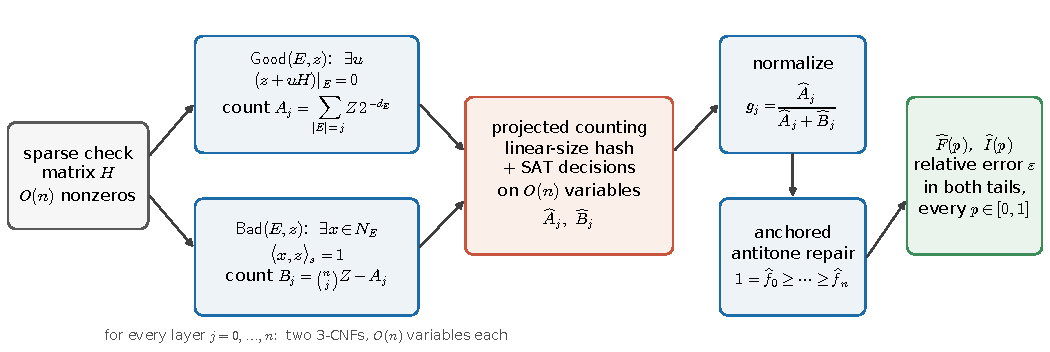
\includegraphics[width=\textwidth]{figures/pipeline.pdf}
\caption{The reduction. For each erasure weight \(j\), two existential
certificates over the same pairs \((E,z)\) have complementary projected
counts \(A_j\) and \(B_j\). Each count is estimated by hashing with a
linear-size circuit and SAT decisions on \(O(n)\) variables. Normalizing
the two estimates and repairing the shape gives one coefficient vector
that controls the fidelity and the infidelity curve at once.}
\label{fig:pipeline}
\end{figure}

The Lean-verified theorem of OpenAI~\cite{openai2026eth} supplies a
polynomial-space engine with running time
\(2^{O(v(\log\log v)^2/\sqrt{\log v})}\) on \(v\) variables.
Corollary~\ref{cor:unconditional} then gives an unconditional algorithm
with the same rate in \(n\) and
polynomial space; the reduction, the engine and their composition are
machine-checked (Section~\ref{sec:formal}), so the corollary rests on no
unrefereed proof. Remarks~\ref{rem:sharp} and~\ref{rem:anthropic} give
the rate \(2^{O(n/\sqrt{\log n})}\) under two further instantiations.

\paragraph{Why both tails, and why a SAT oracle.}
Relative approximation of \(F_H\) alone is easy near \(p=0\), where
\(F_H\approx1\); relative approximation of \(I_H\) alone is easy near
\(p=1\). The content of the guarantee is that one coefficient vector
controls both, including a tail that may be \(e^{-\Theta(n)}\). In the
classical theory of network reliability the two tails are genuinely
different problems, with separate approximation
schemes~\cite{karger1999,guojerrum2019} and in one case a hardness
separation~\cite{fengguo2023,fengfuguo2026}. Here a single counting event
gives both, because the per-pattern fidelity \(2^{-d_E}\) and infidelity
\(1-2^{-d_E}\) are the fractions of \emph{complementary} projected sets
of the same size \(|N|\) (Proposition~\ref{prop:cert}).

The oracle is needed. Proposition~\ref{prop:distance} shows that
\emph{any} output meeting the two-tail guarantee with \(\eps<1\)
determines the minimum distance of the code: the first nonzero
infidelity coefficient sits at index \(d\). Computing the distance of a
stabilizer code is NP-hard~\cite{kapshikarkundu2023,vardy1997}, and
appending qubits that each carry a single-qubit check makes any
presentation sparse without changing the curve
(Corollary~\ref{cor:sparsehard}). So for every sparsity constant \(c>1\)
no polynomial-time algorithm meets the guarantee unless
\(\mathrm{NP}\subseteq\mathrm{BPP}\). The hardness is already present at
a single point: one value \(I_H(p)\) at an explicitly given small \(p\),
known only up to an exponentially large factor, determines the distance
(Proposition~\ref{prop:point}). What remains open is a
\emph{fine-grained} lower bound, since the padding is not
size-preserving, and hardness for presentations of bounded row and
column weight (Section~\ref{sec:limits}).

\paragraph{Why approximate rather than count.}
The external engine counts models exactly. We nonetheless reduce to
\emph{decision} and approximate, because the certificates are not
parsimonious: the number of witnesses of a positive instance depends on
\(E\) (Proposition~\ref{prop:cert}), so witness totals are not the
counts that define the curve. Projected counting onto the bits \((E,z)\)
removes the multiplicity, and hashing-based projected counting needs
only a decision oracle and keeps every query linear in \(n\)
(Appendix~\ref{app:counter}).

\paragraph{Contributions.}
\begin{enumerate}
\item \emph{Complementary projected certificates with linear incidence}
 (Section~\ref{sec:quantum}). Two existential predicates on
 \((E,z)\), \(z\) in the normalizer \(N\), whose counts are
 \(|N|2^{-d_E}\) and \(|N|(1-2^{-d_E})\), each a projection of a 3-CNF
 with \(O(n+\mathrm{nnz}(H))\) variables and clauses, where
 \(\mathrm{nnz}(H)\) is the number of nonzero entries of \(H\). This is a
 projected use of cleaning duality~\cite{bravyiterhal2009,kalachevsadov2022};
 it needs no logical-operator basis and no rank computation inside the
 circuit.
\item \emph{A linear-size transfer with no loss in the shape step}
 (Sections~\ref{sec:transfer} and~\ref{sec:latent},
 Appendices~\ref{app:hash} and~\ref{app:counter}). An all-length
 adaptation of the linear-size pairwise-independent hash of
 Ishai, Kushilevitz, Ostrovsky and Sahai~\cite{ikos2008} keeps every SAT
 query at \(O(n)\) variables of bounded clause density, and an anchored
 antitone repair on a finite partial order (Lemma~\ref{lem:repair})
 restores monotone shape and exact endpoints while preserving the
 two-tail relative interval exactly. The same lemma handles the iid
 case, the uncorrectable-erasure probability, monotone latent circuits
 and the multiclass tensor case.
\item \emph{An end-to-end machine-checked complexity bound}
 (Section~\ref{sec:formal}). The reduction is formalized as a concrete
 multitape machine whose run, output, time and space are proved in
 Lean~4; the external verified SAT engine is linked through proved
 encoding and resource bridges in a single 6{,}157-module graph, so that
 the final statements have no SAT, hashing or solver hypothesis. To our
 knowledge this is the first machine-checked time and space bound for an
 algorithm that calls a machine-checked subexponential SAT engine.
\end{enumerate}
We also give the hardness side (distance determination from the curve
and from a single value, and NP-hardness for sparse presentations
through a direct reduction from SAT to the distance of a CSS code with
one logical qubit, whose correctness is machine-checked), an exact separation showing that ordinary weight enumerators
do not determine the curve, a sampling-model lower bound, extensions to
correlated erasures generated by linear-size circuits from latent bits,
including a fixed number of latent probability classes with a
multivariate monotone output (Theorem~\ref{thm:multiclass}), and
computed examples on codes of up to 128 qubits
(Section~\ref{sec:computed}).

\paragraph{Scope.}
The theorems are asymptotic: they establish the fine-grained transfer
from satisfiability to the erasure curve, and
Section~\ref{sec:computed} supplies the estimator for real codes, a
hybrid whose error bars are statistical. The results concern flagged
erasure of stabilizer codes with a maximally mixed logical input. The
constants, the exact extent of the formalization and the open problems
are collected in Sections~\ref{sec:formal} and~\ref{sec:limits}.

\section{Model and objective}
\label{sec:model}

Fix a constant \(c>0\). The input is a binary check matrix \(H\) with
\(2n\) columns and at most \(cn\) nonzero entries. Its row space \(S\) is
isotropic for the standard symplectic form on \(W=\F^{2n}\).
Delete zero rows, but retain arbitrary remaining redundancies. Write
\[
 s=\dim S,\qquad k=n-s,\qquad N=S^\perp,\qquad Z=|N|=2^{2n-s}.
\]
A consistent choice of stabilizer signs defines an \([[n,k]]\) code;
the quantities studied here do not depend on that choice.
For each qubit, independently, erasure occurs with the same probability
\(p\). The recovery receives the erased set as a classical flag.

Let \(D=2^k\), let \(\Phi_D\) be the normalized maximally entangled state
of a logical system and a reference, and let \(\mathcal N_{H,p}\) be the
channel that encodes the logical system, erases each qubit independently
with probability \(p\) by replacing it with a fixed state and recording
the erased set in a classical flag register. Define
\begin{equation}\label{eq:objective}
 F_H(p)=\max_{\mathcal R}
 \langle\Phi_D|(\operatorname{id}\otimes
  \mathcal R\circ\mathcal N_{H,p})(|\Phi_D\rangle\langle\Phi_D|)
 |\Phi_D\rangle,\qquad I_H(p)=1-F_H(p).
\end{equation}
The maximum is over all CPTP recoveries to the logical system that may
read the flag. Thus \(F_H\) is the entanglement fidelity for the
maximally mixed logical input; throughout, ``entanglement fidelity''
means this squared overlap. It is not worst-case fidelity, and it is not
the probability that the erased region is perfectly correctable.

\paragraph{What the curve measures.}
An erased region is perfectly correctable exactly when \(d_E=0\)
(Section~\ref{sec:quantum}). The probability \(U_H(p)=\Prob(d_E>0)\) of an
uncorrectable pattern therefore differs from \(I_H(p)\), although
\[
 I_H(p)\le U_H(p)\le2I_H(p).
\]
Indeed \(1-2^{-d_E}\) is zero when \(d_E=0\) and belongs to
\([1/2,1]\) otherwise; the comparison is noted
in~\cite{ashikhmin2020}, where \(U_H\) is the decoding-error probability
\(P_{de}\). This constant-factor relation is not an
\(\eps\)-relative approximation of \(U_H\).
For an optimal syndrome/Pauli recovery, \(2^{-d_E}\)
is the probability of selecting the correct logical class in the
induced Pauli mixture, so \(I_H(p)\) is the logical error rate of the
maximum-likelihood erasure decoder with uniform tie-breaking. That event
supplies no herald of successful recovery. The Haar-average pure-state
fidelity is instead \((DF_e+1)/(D+1)\), where \(F_e\) is the
entanglement fidelity of~\eqref{eq:objective} and \(D=2^k\). For one erased repetition-code
qubit these three quantities are, respectively, correctability zero,
entanglement fidelity \(1/2\), and average fidelity \(2/3\).
Corollary~\ref{cor:uncorrectable} approximates \(U_H\) directly.

\section{Main results}
\label{sec:results}

\begin{theorem}[Quantitative transfer]\label{thm:main}
Let \(T\colon\mathbb N\to\mathbb N\) be nondecreasing, and suppose that
for some fixed clause density \(\Delta>0\) there is a deterministic algorithm
that decides satisfiability of 3-CNFs with \(v\) variables and at most
\(\Delta v\) clauses in time \(\poly(\ell)\,T(v)\) and space \(\poly(\ell+v)\),
where \(\ell\) is the length of the binary encoding of the formula.
Then there is a randomized algorithm that, given \(H\) as in
Section~\ref{sec:model} and rational \(0<\eps,\delta<1\), returns
rational coefficients
\[
 1=\widehat f_0\ge\widehat f_1\ge\cdots\ge
 \widehat f_n=4^{-k}
\]
such that, writing
\[
 \widehat F(p)=\sum_{j=0}^n\widehat f_j\Bern{n}{j},
 \qquad
 \widehat I(p)=\sum_{j=0}^n(1-\widehat f_j)\Bern{n}{j},
\]
with probability at least \(1-\delta\), simultaneously for every real
\(p\in[0,1]\),
\begin{equation}\label{eq:guarantee}
 |\widehat F(p)-F_H(p)|\le\eps F_H(p),\qquad
 |\widehat I(p)-I_H(p)|\le\eps I_H(p).
\end{equation}
Every run produces curves in \([0,1]\) with exact endpoints,
\(\widehat F+\widehat I=1\), nonincreasing \(\widehat F\), and
nondecreasing \(\widehat I\). Zero infidelity coefficients are identified
deterministically and retained exactly.

Let \(L\) be \(n\) plus the total bit length of the encodings of
\(H,n,\eps,\delta\). The algorithm runs in time
\[
 \poly(L,\eps^{-1},\log\delta^{-1})\,T(C_cn)
\]
for a constant \(C_c\) depending only on \(c\), and in space polynomial
in \(L\). The case \(n=0\) is returned directly.
\end{theorem}

\begin{proposition}[Resource accounting]\label{prop:resources}
In Theorem~\ref{thm:main}, for \(n\ge1\), the algorithm makes
\(O(n^3\eps^{-2}\log((n+1)/\delta))\) SAT queries, each a 3-CNF with
\(O_c(n)\) variables and \(O_c(n)\) clauses, and each output coefficient
has \(O(n+\log\eps^{-1})\) bits. The clause density of the queries is
bounded by a constant depending only on \(c\), independent of
\(\eps,\delta\); a bound for any specified positive density suffices
after padding queries with unused variables at a constant-factor cost.
The time bound of Theorem~\ref{thm:main} uses only the time premise on
the SAT algorithm; the space bound uses the space premise.
\end{proposition}

The input-length convention includes reading long rational precision
parameters, even when their numerical values remain bounded; without it
the polynomial prefactor would omit the cost of reading \(\eps,\delta\).

\paragraph{Instantiations.}
The following external results supply \(T\). We separate what is
machine-checked from what is claimed.

\begin{corollary}[Unconditional instantiation]\label{cor:unconditional}
There is a randomized algorithm with the guarantees of
Theorem~\ref{thm:main} running in time
\begin{equation}\label{eq:formalrate}
 \poly(L,\eps^{-1},\log\delta^{-1})\,
 2^{O_c(n(\log\log n)^2/\sqrt{\log n})}
\end{equation}
and polynomial space.
\end{corollary}
\begin{proof}
The Lean-verified theorem
\lean{SqrtLogSpace.sat\_polynomial\_space} of~\cite{openai2026eth}
(commit \texttt{4eaee875}; see Section~\ref{sec:formal}) gives, for every
\(k\ge3\), a fixed machine that decides satisfiability of width-\(k\)
CNFs on \(v\) variables with formula bit length \(\ell\) in time at most
\(C(\ell+1)^d2^{A\rho(v)}\), where
\(\rho(v)=v(\ln\ln(v+16))^2/\sqrt{\ln(v+16)}\), with every execution
prefix visiting at most \(S(\ell+1)^e\) cells. Put
\(T(v)=\max_{s\le v}\lceil2^{A\rho(s)}\rceil+1\), which is nondecreasing.
Apply Theorem~\ref{thm:main}.
\end{proof}

The corollary is unconditional in the sense that every hypothesis is a
kernel-checked theorem; Section~\ref{sec:formal} records that the
composition of the reduction with this engine has itself been checked,
including the translation between the engine's input convention and ours.

\begin{remark}[Sharper conditional rate]\label{rem:sharp}
The manuscript~\cite{openai2026eth} also claims, in an appendix that is
not part of its Lean development, that bounded-density \(k\)-SAT is
decidable in polynomial space and time
\(2^{O(n/\sqrt{\log n})}\). If that claimed algorithm is correct, then
Theorem~\ref{thm:main} gives time
\begin{equation}\label{eq:sharp}
 \poly(L,\eps^{-1},\log\delta^{-1})\,
 2^{O_c(n/\sqrt{\log n})}
\end{equation}
with polynomial space. We do not rely on this rate anywhere else.
\end{remark}

\begin{remark}[Time-only rate from a second verified engine]
\label{rem:anthropic}
The Lean-verified main theorem of~\cite{anthropic2026sat} decides
\(k\)-CNFs with \(m\) clauses on \(n\) variables, and counts their
models, in time
\(2^{C\min\{km/\sqrt{\log m},\;k^2n\log\log n/\sqrt{\log n}\}}\) on
Mathlib's multi-stack machine model, with no space bound. Our queries,
after deletion of unused variables and duplicate clauses, have
\(m=O(v)\), so the time bound of Theorem~\ref{thm:main} becomes
\(\poly\cdot2^{O_c(n/\sqrt{\log n})}\) with no space bound. This is a
paper-level observation: that machine model has not been connected
formally to ours.
\end{remark}

\begin{remark}[Comparison with the trivial algorithm]\label{rem:crossover}
Exhaustive enumeration takes \(2^n\poly(n)\) time and polynomial space.
The bound~\eqref{eq:formalrate} improves on it only once
\(C_cA\,(\log\log n)^2/\sqrt{\log n}<1\), that is, for
\(n>2^{\Theta((C_cA)^2)}\) up to log-log factors. With the constants of
the formalized construction (Section~\ref{sec:limits}) that crossover is
astronomically large. The contribution is the fine-grained transfer;
Section~\ref{sec:computed} gives an estimator for real codes.
\end{remark}

\section{Sparse positive representations of both tails}
\label{sec:quantum}

For \(E\subseteq[n]\), let \(V_E\subset W\) be the subspace of Pauli
vectors supported on \(E\). Put
\[
 N_E=N\cap V_E,\qquad S_E=S\cap V_E,\qquad
 d_E=\dim N_E-\dim S_E.
\]
The image of \(N_E\) in \(N/S\) has dimension \(d_E\), so
\(0\le d_E\le2k\).

\begin{lemma}[Known fixed-erasure optimum]\label{lem:fidelity}
For fixed \(E\), the optimum in~\eqref{eq:objective} is
\(F_{\mathrm{opt}}(E)=2^{-d_E}\). Consequently
\(F_H(p)=\E_E[2^{-d_E}]\).
\end{lemma}
\begin{proof}
Erasure is recovery-equivalent to replacing the erased subsystem by
the maximally mixed state: one simulation appends that fixed state,
and the other discards it. The replacement is the uniform mixture of
the \(4^{|E|}\) Pauli errors in \(V_E\).
The syndrome map on \(V_E\) has kernel \(N_E\). Each reachable syndrome
therefore has \(2^{d_E}\) equally likely logical classes, since two
errors in its fibre have the same logical action precisely when their
difference is in \(S_E\).

For completeness, optimization over all CPTP maps follows from
Pauli orthogonality, not a restriction on the decoder. Write a general
encoded Pauli channel with Kraus operators
\(\sqrt{p_{q,\ell}}V_qL_\ell\), where \(q\) is a syndrome,
\(V_q\) maps the logical space isometrically into its syndrome sector,
and the \(D^2\) logical Paulis \(L_\ell\) form an orthogonal unitary basis.
For arbitrary recovery Kraus operators \(R_a\), put \(M_{a,q}=R_aV_q\).
Trace preservation and Parseval give
\[
 \sum_aM_{a,q}^\dagger M_{a,q}=I_D,\qquad
 \sum_\ell|\tr(ML_\ell)|^2=D\tr(M^\dagger M).
\]
Thus
\[
 F_e=D^{-2}\sum_{a,q,\ell}p_{q,\ell}
       |\tr(M_{a,q}L_\ell)|^2
 \le\sum_q\max_\ell p_{q,\ell}.
\]
Syndrome measurement followed by a maximizing logical correction
attains this bound, as in~\cite[Appendix A]{fsw2008}.
For erasure the conditional maximum is \(2^{-d_E}\).
Orthogonal classical erasure flags permit independent optimal
recoveries for every \(E\), proving the expectation formula.
\end{proof}

The inverse-rank expression appears explicitly in
\cite[Eqs.~(17)--(18)]{gullans2021} and, in equivalent form, in the
erasure-channel analysis of~\cite{delfossezemor2013},
in~\cite[Section~III]{ashikhmin2020} as the reciprocal of the number of
logical classes that have a representative supported on the erased set,
and in the degenerate-decoding analysis of~\cite{kuoouyang2026}. It gives fidelity
one for empty erasure, \(4^{-k}\) for full erasure, and one for every
erasure when \(k=0\). The exponent \(d_E\) can be odd. For example, one
erased qubit of the three-qubit repetition code has \(d_E=1\).

\begin{proposition}[Complementary projected certificates]\label{prop:cert}
Let \(m\) be the number of retained rows of \(H\). For \(z\in N\), define
\begin{align*}
 \Good(E,z)&\iff
    \exists u\in\F^m:\ (z+uH)|_E=0,\\
 \Bad(E,z)&\iff
    \exists x\in N_E:\ \pair{x}{z}=1.
\end{align*}
These predicates are complementary, and
\begin{equation}\label{eq:counts}
 \#\{z\in N:\Good(E,z)\}=Z2^{-d_E},\qquad
 \#\{z\in N:\Bad(E,z)\}=Z(1-2^{-d_E}).
\end{equation}
A positive Good instance has \(2^{m-\rank H_E}\) coefficient witnesses,
where \(H_E\) retains both columns of each qubit in \(E\).
A positive Bad instance has \(|N_E|/2\) witnesses.
\end{proposition}
\begin{proof}
Nondegenerate finite-dimensional orthogonality gives
\[
 (N\cap V_E)^\perp=N^\perp+V_E^\perp=S+V_{\bar E}.
\]
Thus \(z\) annihilates \(N_E\) exactly when it differs from a vector
\(uH\in S\) by a vector supported outside \(E\), precisely Good.
Over \(\F\), failure to annihilate means pairing to one with some
\(x\in N_E\), precisely Bad. This logical equivalence holds even for
\(z\in W\); the count in~\eqref{eq:counts} uses \(z\in N\).

Consider \(\phi_E:N\to N_E^*\), with
\(\phi_E(z)(x)=\pair{x}{z}\). The transpose map \(N_E\to N^*\) has
kernel \(N_E\cap N^\perp=N_E\cap S=S_E\), using \(S\subseteq N\).
The two maps have equal rank, so \(\rank\phi_E=d_E\) and
\[
 |\ker\phi_E|=2^{\dim N-d_E}=Z2^{-d_E}.
\]
Good is this kernel and Bad its complement in \(N\).
Finally \(u\mapsto(uH)|_E\) has rank \(\rank H_E\), giving the
first fibre size. For a positive Bad instance,
\(x\mapsto\pair{x}{z}\) is a nonzero linear functional on \(N_E\),
giving the second.
\end{proof}

This is a projected use of cleaning/annihilator
duality~\cite{bravyiterhal2009,kalachevsadov2022}.
Its counting domain and projection are essential. For a Bell stabilizer
state under full erasure, Good has probability one over \(N=S\), but
probability \(1/4\) over the ambient \(W\). Nor can one simply count
witnesses: for a Bell pair on qubits \(1,2\) and two free qubits,
the weight-two erasures \(\{1,3\}\) and \(\{3,4\}\) give, respectively,
two and eight witnesses per positive Bad pair. This \(E\)-dependent
multiplicity is why Section~\ref{sec:transfer} counts projected
assignments with a decision oracle rather than witnesses with a counting
oracle.

\begin{lemma}[Linear incidence]\label{lem:cnf}
For each \(j\), the predicates
\((|E|=j,z\in N,\Good(E,z))\) and
\((|E|=j,z\in N,\Bad(E,z))\) are projections onto the \(3n\) bits
\((E,z)\) of 3-CNFs with \(O(n+w)\) variables and clauses, where
\(w\) is the number of nonzero entries of \(H\).
They are constructible in polynomial time.
\end{lemma}
\begin{proof}
Write \(H=(H_X\mid H_Z)\). Membership in \(N\) is the row-parity
system \(H_Xz_Z+H_Zz_X=0\), computed by \(O(w)\) XOR gates.
For Good, columnwise XOR chains compute \(uH\) with \(O(w)\) gates,
and \(2n\) implications require equality with \(z\) on erased qubits.
There are \(m\le w\) coefficient-witness bits.
For Bad, repeat the row checks for \(x\), impose \(2n\) support
implications, and compute the symplectic pairing using \(2n\) AND
gates and an XOR chain.

A carry-save population counter imposes \(|E|=j\) with \(O(n)\)
gates. Each three-to-two compressor reduces the total live-bit count
by one; after at most \(n\) compressions, a ripple addition and
comparison use \(O(\log n)\) gates. Full-equivalence Tseitin
clauses for binary gates have width at most three and constant size.
Existentially quantify the witnesses and all gate auxiliaries,
leaving only \(E,z\) projected. Both gate and wire counts are linear.
\end{proof}

Let \(A_j,B_j\) be the two projected counts in Lemma~\ref{lem:cnf}.
Proposition~\ref{prop:cert} implies
\begin{align}
 A_j+B_j&=\binom njZ,\qquad
 f_j=\frac{A_j}{\binom njZ},\label{eq:layers}\\
 F_H(p)&=Z^{-1}\sum_{j=0}^n A_jp^j(1-p)^{n-j},&
 I_H(p)&=Z^{-1}\sum_{j=0}^n B_jp^j(1-p)^{n-j}.\label{eq:positive}
\end{align}
There is no extra binomial factor in~\eqref{eq:positive}: the counts
already include every set of size \(j\). Every \(A_j>0\), since
\(z=0\) is Good for every \(E\).

\section{From projected counts to both reliability curves}
\label{sec:transfer}

The following counting tool supplies the quantitative budget.
Its all-length hash construction and proof are given in the appendices;
the estimator is an adaptation of the hashing method of
Stockmeyer~\cite{stockmeyer1985} and Valiant and
Vazirani~\cite{valiantvazirani1986} in the form used by modern
approximate model counters~\cite{gomes2006,cmv2013}.

\begin{proposition}[Projected counting with linear query size]
\label{prop:counter}
For a 3-CNF with \(v\) variables and \(O(v)\) clauses, and a specified
set of \(q\le v\) projection bits, its number of distinct projected
models has a relative-\(\eta\) estimate with confidence \(1-\zeta\)
using \(O((q+1)^2\eta^{-2}\log(1/\zeta))\) SAT calls for
\(0<\zeta\le1/2\). Each query has \(O(v)\) variables and clauses.
Zero counts are detected deterministically, and positive counts
always receive positive estimates. The wrapper uses polynomial space.
\end{proposition}

\paragraph{The repair lemma.}
Four places in this paper turn coefficientwise relative estimates into a
monotone output without losing accuracy: the iid case, the
uncorrectable-erasure probability, monotone latent circuits, and the
multiclass tensor case. One lemma covers all of them. For
\(0\le\eps\le1\), write the \emph{two-tail interval} of \(t\in[0,1]\) as
\([L_\eps(t),U_\eps(t)]\), where
\begin{equation}\label{eq:twotail}
 L_\eps(t)=\max\{(1-\eps)t,(1+\eps)t-\eps\},\qquad
 U_\eps(t)=\min\{(1+\eps)t,(1-\eps)t+\eps\}.
\end{equation}
A number \(g\) lies in this interval exactly when
\(|g-t|\le\eps t\) and \(|g-t|\le\eps(1-t)\). Both endpoints are
nondecreasing in \(t\) and enclose \(t\).

\begin{lemma}[Anchored antitone repair]\label{lem:repair}
Let \((J,\le)\) be a finite partial order, let \(f\colon J\to[0,1]\) be
antitone, and let \(\mathrm{lo},\mathrm{hi}\colon[0,1]\to\mathbb R\) be
nondecreasing with \(\mathrm{lo}(t)\le t\le\mathrm{hi}(t)\). Let
\(A\subseteq J\) be a set of anchors with known values
\(v_a=f_a\) for \(a\in A\), and let \(h\colon J\to\mathbb R\) be arbitrary.
Replace \(h_a\) by \(v_a\) for \(a\in A\), clip all other values to
\([0,1]\), and define
\[
 \ell_j=\min_{i\le j}h_i,\qquad
 u_j=\max\bigl(\{0\}\cup\{v_a:a\in A,\ j\le a\}\bigr),
 \qquad \widetilde f_j=\max\{u_j,\ell_j\}.
\]
Then, for every input \(h\), \(\widetilde f\) is antitone with values in
\([0,1]\) and \(\widetilde f_a=v_a\) for every anchor. If moreover
\(h_j\in[\mathrm{lo}(f_j),\mathrm{hi}(f_j)]\) for every \(j\), then
\(\widetilde f_j\in[\mathrm{lo}(f_j),\mathrm{hi}(f_j)]\) for every \(j\).
\end{lemma}
\begin{proof}
If \(j\le j'\) then \(\{i:i\le j\}\subseteq\{i:i\le j'\}\), so
\(\ell_{j'}\le\ell_j\); and \(\{a:j'\le a\}\subseteq\{a:j\le a\}\), so
\(u_{j'}\le u_j\). A maximum of two antitone functions is antitone.
Values lie in \([0,1]\) because the clipped \(h\) and the anchors do.
At an anchor \(a\), every \(v_{a'}\) with \(a\le a'\) satisfies
\(v_{a'}=f_{a'}\le f_a=v_a\), and \(v_a\) itself is among them, so
\(u_a=v_a\); and \(\ell_a\le h_a=v_a\). Hence \(\widetilde f_a=v_a\).

For the interval claim, note first that clipping preserves membership:
if \(h_i>1\) then \(\mathrm{hi}(f_i)\ge h_i>1\ge f_i\ge\mathrm{lo}(f_i)\),
and if \(h_i<0\) then \(\mathrm{lo}(f_i)\le h_i<0\le f_i\le\mathrm{hi}(f_i)\);
anchors satisfy \(v_a=f_a\) trivially. For the lower bound, every
\(i\le j\) has \(f_i\ge f_j\), so
\(h_i\ge\mathrm{lo}(f_i)\ge\mathrm{lo}(f_j)\), whence
\(\ell_j\ge\mathrm{lo}(f_j)\) and \(\widetilde f_j\ge\mathrm{lo}(f_j)\).
For the upper bound, \(\ell_j\le h_j\le\mathrm{hi}(f_j)\); every anchor
\(a\ge j\) has \(v_a=f_a\le f_j\le\mathrm{hi}(f_j)\); and
\(0\le f_j\le\mathrm{hi}(f_j)\). Hence \(u_j\le\mathrm{hi}(f_j)\) and
\(\widetilde f_j\le\mathrm{hi}(f_j)\).
\end{proof}

The lemma makes no use of how \(h\) was produced; the shape and anchor
properties hold on every run, and accuracy is preserved on the event
that the input was accurate. With \((J,\le)=(\{0,\ldots,n\},\le)\),
anchors \(\{0,n\}\) and the endpoints~\eqref{eq:twotail}, the rule reads
\(\widetilde f_j=\max\{f_n,\min_{i\le j}h_i\}\), where \(h_0\) and \(h_n\)
have first been replaced by \(f_0\) and \(f_n\). The replacement is part
of the rule: without it the running minimum at \(j=n\) could exceed
\(f_n\). A nondecreasing target is handled by applying the
lemma to \(1-f\). Monotone rearrangement of confidence bands is a
classical device in shape-constrained
estimation~\cite{robertson1988,chernozhukov2009}; the point here is that
the \emph{multiplicative} two-tail interval is preserved with no
additional failure allowance.

\begin{proof}[Proof of Theorem~\ref{thm:main}]
Apply Proposition~\ref{prop:counter} to all \(2(n+1)\) counts with
\[
 \eta=\eps/3,\qquad \zeta=\delta/[2(n+1)].
\]
With probability at least \(1-\delta\), every estimate is relatively
accurate. On this single event, set
\[
 g_j=\frac{\widehat A_j}{\widehat A_j+\widehat B_j}.
\]
Both fidelity and infidelity must be controlled after this normalization.
For \(f=A/(A+B)\in(0,1)\), write
\(\alpha=\widehat A/A,\ \beta=\widehat B/B\).
Then
\begin{equation}\label{eq:normalization}
 g-f=\frac{f(1-f)(\alpha-\beta)}
                {f\alpha+(1-f)\beta}.
\end{equation}
Since \(\alpha,\beta\in[1-\eta,1+\eta]\), both relative errors
are at most
\[
 \frac{2\eta}{1-\eta}=\frac{2\eps}{3-\eps}\le\eps,
\]
that is, \(g_j\in[L_\eps(f_j),U_\eps(f_j)]\).
Exact zeros handle \(f=0,1\). The denominator is positive on every
run because every Good count receives a positive estimate.
The tolerance slack is real: choosing \(\eta=\eps/2\) would not
work uniformly. With \(f=1/16,\eps=1/2,\alpha=5/4,\beta=3/4\),
normalization gives \(g=1/10\), a relative fidelity error of \(3/5\).

Next, the image of \(N_E\) in \(N/S\) is nested under inclusion of
\(E\). Hence \(d_E\) increases and \(2^{-d_E}\) decreases under
inclusion. Coupling uniform sets of consecutive sizes by initial
segments of a uniform permutation shows
\[
 1=f_0\ge f_1\ge\cdots\ge f_n=b,\qquad b=4^{-k}.
\]
Apply Lemma~\ref{lem:repair} on \(\{0,\ldots,n\}\) with anchors
\(\{0,n\}\), values \(1\) and \(b\), input \(h=g\), and the
endpoints~\eqref{eq:twotail}. Writing \(\bar g\) for \(g\) with the two
anchor entries replaced, the rule is
\begin{equation}\label{eq:repair}
 \widehat f_j=\max\bigl\{b,\min_{i\le j}\bar g_i\bigr\},\qquad
 \bar g_0=1,\quad \bar g_n=b,\quad \bar g_i=g_i\ \ (0<i<n).
\end{equation}
In particular \(\widehat f_0=1\) and \(\widehat f_n=b\); no clipping is
needed because every \(g_i\) is a ratio in \([0,1]\).
By the lemma, \(\widehat f\) is nonincreasing with exact endpoints on
every run, and on the accuracy event both relative bounds hold for
every \(\widehat f_j\).

Multiply the layerwise inequalities by the nonnegative Bernstein
weights and sum to obtain~\eqref{eq:guarantee} for every real \(p\)
on that same event. No discretization or union bound over \(p\) is
needed. The weights sum to one, giving complementarity and range.
Monotonicity of the curve follows from
\[
 \widehat F'(p)=n\sum_{j=0}^{n-1}
  (\widehat f_{j+1}-\widehat f_j)\Bern{n-1}{j}\le0.
\]

Zero infidelity layers are an initial segment. Their exact SAT zero
tests give \(g_j=1\), which the repair retains. If \(k>0\), positive
\(B_j\) gives \(g_j<1\) and \(b<1\), so the repair invents no extra
zero layer. These zero layers are exactly \(j<d\), with \(d\) the
minimum nontrivial logical weight: a weight-\(d\) logical support
can be extended to an erased set of any size \(j\ge d\).
For \(k=0\), the output is identically \((1,0)\).

The resource claims are Proposition~\ref{prop:resources}, proved next.
\end{proof}

\begin{proof}[Proof of Proposition~\ref{prop:resources}]
Here \(q=3n\). The query count follows by multiplying the bound in
Proposition~\ref{prop:counter} by \(2(n+1)\); query sizes follow
from Lemma~\ref{lem:cnf} together with the \(O(q)\) hash variables and
clauses of Lemma~\ref{lem:hash}. Accuracy affects the number of calls,
not the query size. The queries have \(O_c(n)\) clauses on \(O_c(n)\)
variables, so their density is bounded by a constant depending on \(c\)
alone; padding with unused variables lowers the density to any
prescribed positive value at constant-factor cost. Sequential processing
of the queries gives polynomial space for the wrapper; the total space
is the wrapper's plus the SAT algorithm's, which is where the space
premise enters, and nowhere else. The estimator's integer outputs have
\(O(n+\log\eps^{-1})\) bits, and normalization, exact endpoints and
running minima preserve this bit bound. Evaluation at rational \(p\) has
polynomial additional bit cost in its encoding length. The time bound is
the number of queries times \(\poly(\ell)T(v)\) with \(v=O_c(n)\) and
\(\ell=\poly(L)\), plus polynomial work, and uses only the time premise
and the monotonicity of \(T\).
\end{proof}

\section{Hardness and comparisons}
\label{sec:hardness}

\subsection{Any accurate output determines the distance}

Let \(k>0\) and let \(d\) be the minimum weight of a nontrivial logical
operator, that is, the least \(|E|\) with \(d_E>0\).

\begin{proposition}[Distance determination]\label{prop:distance}
Let \(0\le\eps<1\) and let \(\widehat I(p)=\sum_{j=0}^nc_j\Bern{n}{j}\)
with all \(c_j\ge0\) satisfy \(|\widehat I(p)-I_H(p)|\le\eps I_H(p)\)
for every \(p\in[0,1]\). Then \(c_j=0\) for \(j<d\) and \(c_d>0\).
In particular \(d=\min\{j:c_j>0\}\), and the order of vanishing of
\(\widehat I\) at \(p=0\) equals \(d\).
\end{proposition}
\begin{proof}
By~\eqref{eq:positive}, \(I_H(p)=Z^{-1}\sum_{j\ge d}B_jp^j(1-p)^{n-j}\)
with \(B_d>0\) and \(B_j=0\) for \(j<d\), so
\(I_H(p)=(B_d/Z)p^d(1+O(p))\) as \(p\to0^+\). The hypothesis gives
\((1-\eps)I_H\le\widehat I\le(1+\eps)I_H\), hence
\(\widehat I(p)/p^d\) stays between \((1-\eps)B_d/Z>0\) and
\((1+\eps)B_d/Z<\infty\) for small \(p>0\). If some \(c_j>0\) with
\(j<d\), then \(\widehat I(p)/p^d\ge c_j\binom nj(1-p)^{n-j}p^{j-d}\to\infty\),
a contradiction. If \(c_j=0\) for all \(j\le d\), then
\(\widehat I(p)/p^d\to0\), a contradiction. Hence \(c_j=0\) for \(j<d\)
and \(c_d>0\).
\end{proof}

The proof uses the hypothesis only for small \(p>0\). Nonnegativity of
the \(c_j\) is a convenience: for coefficients of arbitrary sign, the
order of vanishing of \(\widehat I\) at \(p=0\) is the index of its
first nonzero Bernstein coefficient, and the two-sided bound forces
that order to be \(d\), so the first nonzero coefficient again sits at
index \(d\).

Consequently, any algorithm meeting the guarantee of
Theorem~\ref{thm:main} with some fixed \(\eps<1\) and \(\delta<1/2\)
computes the minimum distance with probability greater than \(1/2\), by
reading off the first positive infidelity coefficient. The minimum
distance of a stabilizer code is NP-hard to
compute~\cite{kapshikarkundu2023}, as it is for classical linear
codes~\cite{vardy1997,bmvt1978}, and hard to
approximate~\cite{gjs2025,kapshikar2026}. Those proofs reduce from the
classical minimum-distance problem. For the purposes of this paper a
shorter route is available, which we give in full because it is
self-contained and machine-checked: a direct reduction from CNF
satisfiability.

\paragraph{A direct reduction from SAT.}
Let \(\varphi\) be a CNF formula with variables \(x_1,\dots,x_V\) and
nonempty clauses (a formula with an empty clause is replaced by
\(x_1\wedge\neg x_1\)), and let \(K\) be its number of literal
occurrences. For an occurrence \(o\) write \(v(o)\) for its variable and
\(\nu_o=1\) if it is negated, \(\nu_o=0\) otherwise.

\emph{Step A: a linear system.} Take \(2V+3K\) binary coordinates
\(p_i,n_i\) (\(i\le V\)) and \(\sigma_o,w_o,c_o\) (one triple for each
occurrence \(o\)), and the equations over \(\F\)
\[
 p_i+n_i=1,\qquad \sum_{o\in C}\sigma_o=1\ \ (\text{each clause }C),\qquad
 w_o+\sigma_o+p_{v(o)}=\nu_o,\qquad c_o+p_{v(o)}=1+\nu_o ,
\]
written \(Ax=s\). Put \(b_o=p_{v(o)}+\nu_o\), the value of the literal.
Since \(n_i=1+p_i\), \(w_o=\sigma_o+b_o\) and \(c_o=1+b_o\), every
solution has weight
\[
 \operatorname{wt}(x)=V+K+2\,\bigl|\{o:\sigma_o=1,\ b_o=0\}\bigr| :
\]
each pair \((p_i,n_i)\) contributes \(1\), and each triple
\((\sigma_o,\sigma_o+b_o,1+b_o)\) contributes \(1\), or \(3\) when
\(\sigma_o=1\) and \(b_o=0\). If \(a\) satisfies \(\varphi\), set
\(p_i=a_i\) and \(\sigma_o=1\) on one true literal of each clause; the
weight is \(V+K\). Conversely, read an assignment off the \(p_i\): a
clause that it falsifies has \(b_o=0\) on all its occurrences while
\(\sum_{o\in C}\sigma_o=1\), so the weight is at least \(V+K+2\). Hence
the minimum weight of a solution is \(V+K\) if \(\varphi\) is
satisfiable and at least \(V+K+2\) otherwise. The kernel of \(A\) is
spanned by the explicit vectors
\(P_i=p_i+n_i+\sum_{v(o)=i}(w_o+c_o)\) and
\(D_o=\sigma_{o_0}+\sigma_o+w_{o_0}+w_o\), where \(o_0\) is the first
occurrence in the clause of \(o\).

\emph{Step B: the code.} Let \(t=V+K\). Add one coordinate \(\ast\) to
the \(2V+3K\) coordinates, for the column \(s\) of \([A\mid s]\), and
repeat every coordinate \(g\) on \(t+2\) qubits
\((g,0),\dots,(g,t+1)\); there are \(n=(2V+3K+1)(V+K+2)\) qubits. The
stabilizer is generated by (i) \(X\) on copy \(0\) of the supports of
the \(P_i\) and \(D_o\); (ii) \(X_{(g,0)}X_{(g,l)}\) for all \(g\) and
\(l\); (iii) for each equation \(r\) of \(Ax=s\), \(Z\) on all copies of
its support and, if \(s_r=1\), on all copies of \(\ast\). The generators
commute: those of (i) are orthogonal to the rows of \(A\), and those of
(ii) meet each \(Z\)-generator in zero or two qubits. The check matrix
has \(O((V+K)^3)\) nonzero entries.

\begin{proposition}[Distance from satisfiability]\label{prop:satdistance}
The code of \(\varphi\) has exactly one logical qubit. If \(\varphi\) is
satisfiable its distance is \(t+1\); otherwise it is at least \(t+2\). Equivalently, an
uncorrectable erased set of size at most \(t+1\) exists if and only if
\(\varphi\) is satisfiable.
\end{proposition}
\begin{proof}
If \(Ax=s\), the operator \(X\) on \(\{(g,0):x_g=1\}\cup\{(\ast,0)\}\)
commutes with (iii), and it is not in \(S\): the \(X\)-parity on the
copies of \(\ast\) vanishes on every generator and equals one on it. Its
weight is \(\operatorname{wt}(x)+1\), which is \(t+1\) for the solution
of a satisfying assignment. A solution exists because no clause is
empty, so \(k\ge1\). Conversely, let \(X^aZ^b\in N\setminus S\). The
code is CSS, so \(X^a\) and \(Z^b\) are in \(N\) and one of them is not
in \(S\). If \(Z^b\notin S\), then \(b\ne0\), and commutation with (ii)
makes \(b\) constant on the copies of each coordinate, so the weight is
at least \(t+2\). If \(X^a\notin S\), let \(y_g=\sum_la_{(g,l)}\).
Commutation with (iii) gives \(Ay=y_\ast s\) on the original
coordinates. If \(y_\ast=0\), then \(y\in\ker A\), and \(X^a\) is the
product of the lift of \(y\) to copy \(0\), a product of generators (i),
with the generators (ii) at the positions where \(a\) is nonzero; so
\(X^a\in S\), a contradiction. Hence \(y_\ast=1\) and \(y\) solves
\(Ax=s\). Every coordinate with \(y_g=1\), and \(\ast\), carries a
nonzero copy, so the weight is at least \(\operatorname{wt}(y)+1\ge
t+1\), and a weight of at most \(t+1\) forces \(\operatorname{wt}(y)\le
t\), which by Step~A makes \(\varphi\) satisfiable. Finally \(k=1\):
the argument above shows that an \(X\)-type element of \(N\) with
\(y_\ast=0\) is in \(S\), so the \(X\)-type elements of \(N\) form two
classes modulo \(S\); and a \(Z\)-type element of \(N\), after
multiplication by \(Z\) on all copies of \(\ast\) if it anticommutes
with the \(X\)-logical operator, commutes with all of \(N\) and
therefore lies in \(S=N^{\perp}\). Hence \(N\) is generated by \(S\) and
two operators, and \(\dim N-\dim S=2\).
\end{proof}

The code and \(t\) are computed from \(\varphi\) in polynomial time, so
by the Cook--Levin theorem~\cite{cook1971} it is NP-hard to decide
whether the distance of a CSS code with one logical qubit is at most a
given number, and equally whether an uncorrectable erased set of a
given size exists. The reduction combines two known devices. Placing
the kernel of \(A\) in the stabilizer, so that the lightest
\(X\)-logical operator is a minimum-weight coset
element~\cite{bmvt1978}, is the embedding by which Chen and Freedman
show that a shortest nonbounding \(\F\)-cycle is NP-hard to find even
when the homology has rank one~\cite{chenfreedman2011}, and it appears
in the hardness of degenerate decoding~\cite{iyerpoulin2015};
protecting the other logical type by repetition is standard. To our
knowledge this is the first proof that the minimum distance of a
stabilizer code is NP-hard that does not pass through the hardness of
the classical minimum-distance problem~\cite{vardy1997}, on which the
proofs of~\cite{kapshikarkundu2023,gjs2025} rest, and the first that
gives hardness for codes with a single logical qubit. The construction, the
proposition and its composition with Proposition~\ref{prop:distance}
and Proposition~\ref{prop:point} below are formalized
(Section~\ref{sec:formal}); the polynomial running time of the
reduction and the Cook--Levin theorem are not. The codes produced are
not sparse, but sparsity is restored by padding.

\begin{corollary}[Hardness for sparse presentations]\label{cor:sparsehard}
Fix \(c>1\), \(\eps<1\) and \(\delta<1/2\). If a randomized
polynomial-time algorithm meets the guarantee~\eqref{eq:guarantee} of
Theorem~\ref{thm:main} on all check matrices with at most \(cn\) nonzero
entries, then \(\mathrm{NP}\subseteq\mathrm{BPP}\). The same holds for
the relative approximation of \(I_H\) alone, with the output in
Bernstein form as in Proposition~\ref{prop:distance};
Corollary~\ref{cor:pointhard} removes the assumption on the form of the
output.
\end{corollary}
\begin{proof}
Let \(H\) be an arbitrary check matrix on \(n\) qubits with \(w\)
nonzero entries. Append \(n'\) new qubits and, for each of them, one new
row whose only nonzero entry is a \(Z\) on that qubit. The new matrix
\(H'\) has \(n+n'\) qubits and \(w+n'\) nonzero entries, so it satisfies
the sparsity bound as soon as \(n'\ge(w-cn)/(c-1)\), which is polynomial
in the size of \(H\). Its row space is \(S'=S\oplus\langle Z_i\rangle\),
with normalizer \(N'=N\oplus\langle Z_i\rangle\), the sums ranging over
the new qubits \(i\). For \(E\subseteq[n+n']\) the two groups \(N'_E\)
and \(S'_E\) each gain the same factor, generated by the \(Z_i\) with
\(i\in E\) new, so \(d'_E=d_{E\cap[n]}\). Hence \(k\) and the minimum
distance are unchanged and
\(F_{H'}(p)=\E_E\,2^{-d_{E\cap[n]}}=F_H(p)\) identically in \(p\). An
algorithm as in the statement, run on \(H'\), returns with probability
greater than \(1/2\) an output from which
Proposition~\ref{prop:distance} reads off the distance of the code of
\(H\). Applied to the codes of Proposition~\ref{prop:satdistance}, this
decides satisfiability in randomized polynomial time with two-sided
bounded error.
\end{proof}

The padding multiplies the number of qubits by a factor of order
\(w/n\), which is not bounded, so Corollary~\ref{cor:sparsehard} gives
no fine-grained lower bound: it does not show that the curve of an
\(n\)-qubit sparse code needs time \(T(\Omega(n))\). It also says nothing
about presentations in which every row and every column has bounded
weight, where padding is not available. Both questions are open
(Section~\ref{sec:limits}). For \(c\le1\) either some qubit is touched by
no check, or every qubit is touched by exactly one nonzero entry and the
code is a product of single-check blocks. In both cases \(d\le1\)
whenever \(k>0\), so the distance route gives nothing; we do not treat
that regime. Conversely, sparsity enters
Theorem~\ref{thm:main} only through the query size: by
Lemma~\ref{lem:cnf} the same algorithm applies to an arbitrary check
matrix with \(T(C_cn)\) replaced by \(T(C(n+w))\) for an absolute
constant \(C\).

\paragraph{Hardness at a single point.}
Proposition~\ref{prop:distance} uses the whole curve and its Bernstein
form. Neither is needed: one number, at one explicitly given point,
already determines the distance, even when it is known only up to an
exponentially large factor.

\begin{proposition}[A point estimate determines the distance]
\label{prop:point}
Let \(k>0\) and let \(d\) be the minimum distance. For every
\(p\in[0,1]\),
\begin{equation}\label{eq:sandwich}
 \tfrac12\,p^d\le I_H(p)\le\binom nd p^d,
 \qquad
 p^d\le U_H(p)\le\binom nd p^d .
\end{equation}
Consequently, let \(R\ge1\) and \(0<p\le1\) satisfy \(2^{n+1}R^2p<1\),
and let \(\widehat\imath\) be any real number with
\(I_H(p)/R\le\widehat\imath\le R\,I_H(p)\). Then \(d\) is the unique
natural number \(d'\) such that
\[
 \frac{p^{d'}}{2R}\le\widehat\imath\le2^nR\,p^{d'} .
\]
The same holds for \(U_H\) in place of \(I_H\), with the test
\(p^{d'}/R\le\widehat u\le2^nR\,p^{d'}\).
\end{proposition}
\begin{proof}
Let \(E_0\) be an uncorrectable set of size \(d\). Every \(E\supseteq E_0\)
is uncorrectable, so it contributes one to \(U_H\) and at least \(1/2\)
to \(I_H\), and \(\Prob(E\supseteq E_0)=p^d\). Conversely an
uncorrectable set has at least \(d\) elements and therefore contains
some \(d\)-subset, so its indicator is at most the number of
\(d\)-subsets it contains; taking expectations gives
\(U_H(p)\le\binom ndp^d\), and \(I_H\le U_H\). This
proves~\eqref{eq:sandwich}. With \(\binom nd\le2^n\), the true \(d\)
passes the test. If some \(d'<d\) also passed, then
\(p^{d'}/(2R)\le\widehat\imath\le R\,2^np^d\le R\,2^np^{d'+1}\), so
\(1\le2^{n+1}R^2p\); if some \(d'>d\) passed, then
\(p^d/(2R)\le\widehat\imath\le2^nR\,p^{d'}\le2^nR\,p^{d+1}\), with the
same contradiction.
\end{proof}

For example, at \(p=2^{-(n+2r+2)}\), a point with \(O(n+r)\) bits, any
estimate of \(I_H(p)\) within a multiplicative factor \(2^r\) determines
\(d\); a relative error \(\eps<1\) corresponds to the constant
\(R=1/(1-\eps)\). Combined with the padding of
Corollary~\ref{cor:sparsehard}, which changes neither \(I_H\) nor \(d\),
this gives hardness with no assumption on the form of the output:

\begin{corollary}[Pointwise hardness]\label{cor:pointhard}
Fix \(c>1\) and a polynomial \(h\colon\mathbb N\to\mathbb N\), and put
\(p_n=2^{-(n+2h(n)+2)}\). Suppose a randomized polynomial-time algorithm,
given a check matrix \(H\) on \(n\) qubits with at most \(cn\) nonzero
entries, outputs with probability at least \(2/3\) a number
\(\widehat\imath\) with
\(2^{-h(n)}I_H(p_n)\le\widehat\imath\le2^{h(n)}I_H(p_n)\). Then
\(\mathrm{NP}\subseteq\mathrm{BPP}\). The same holds for \(U_H\).
\end{corollary}
\begin{proof}
Given an arbitrary check matrix with \(k>0\), pad it as in
Corollary~\ref{cor:sparsehard} to a matrix \(H'\) on \(n'\) qubits that
meets the sparsity bound; \(n'\) is polynomial, and \(H'\) has the same
\(I_H\), \(U_H\) and \(d\). Run the algorithm on \(H'\) and apply
Proposition~\ref{prop:point} to the code of \(H'\) with
\(R=2^{h(n')}\) and \(p=p_{n'}\), for which \(2^{n'+1}R^2p=1/2\). The
point \(p_{n'}\) has \(O(n'+h(n'))\) bits, and the test of the
proposition, tried for \(d'=1,\ldots,n'\), is polynomial-time arithmetic
on the output. With probability at least \(2/3\) it returns the distance.
Applied to the codes of Proposition~\ref{prop:satdistance}, which have
\(k=1\), and repeated with a majority vote, this decides
satisfiability with two-sided bounded error. For a general input the
case \(k=0\) is recognized by Gaussian elimination.
\end{proof}

Thus the small-\(p\) tail is hard to approximate even within an
exponential factor, for sparse inputs, at a single point. This is the
regime in which Theorem~\ref{thm:main} gives relative error \(\eps\).

\paragraph{What a SAT engine gives exactly.}
The same certificate shows what does \emph{not} need approximation. For
a threshold \(t\), the statement \(d\le t\) is existential,
\[
 d\le t\iff\exists E,\ |E|\le t,\ \exists x\in N_E,\ \exists z\in N:\
 \pair xz=1,
\]
and by Lemma~\ref{lem:cnf} it is the satisfiability of one 3-CNF with
\(O(n+\mathrm{nnz}(H))\) variables, with no projection and no hashing.
A decision algorithm as in Theorem~\ref{thm:main} therefore computes the
distance exactly and deterministically, by binary search over \(t\), in
time \(\poly(L)\,T(O(n+\mathrm{nnz}(H)))\); reductions of the distance to
SAT are standard, and one has been formally
verified~\cite{leanqec2026}. If the algorithm also counts models, as the
verified engine of~\cite{openai2026eth} does, the ordinary weight
enumerators follow exactly as well. The number of \(x\in N\) of weight
\(t\) is the model count of a 3-CNF on the \(2n\) bits of \(x\) in which
every other variable is a function of \(x\): the parity checks for
\(x\in N\), one OR gate per qubit for its support, and a counter for the
weight; no set \(E\) appears. The elements of \(S\) are counted in the
same way through \(x=uH\), with the constant multiplicity \(2^{m-s}\) for
the free choice of \(u\). These are exactly
the quantities that Section~\ref{sec:enumerators} shows do not determine
the curve. The curve weights each erased set by \(2^{-d_E}\), and it is
this weighting that forces the projected, approximate route.

Note that the fidelity tail carries no distance-type obstruction near
\(p=0\): \(\widehat F=1\) is a valid relative approximation of \(F_H\)
there. The obstructions above live in the infidelity tail, which is also
the quantity of practical interest.

\paragraph{Exact evaluation.}
Corollary~\ref{cor:pointhard} with \(h\equiv0\) shows that exact
evaluation of \(I_H\) at the input-dependent point \(p_n=2^{-(n+2)}\) is
NP-hard for sparse presentations. We prove no hardness for exact
evaluation at a fixed constant \(p\), and no \#P-hardness. For a
classical binary linear code the corresponding quantity is the
reliability polynomial of a binary matroid, whose exact evaluation is
\#P-hard~\cite{colbourn1987,britz2002,provanball1983,jvw1990}; the
symplectic-matroid viewpoint is in~\cite{sarvepalli2011}. The quantum
curve is not such a polynomial in disguise: the correctable sets of the
four-qubit CSS code with checks \(ZZIZ,\ XIXX,\ XXXI\) violate the
independent-set exchange axiom, and the weight-two fidelity polynomial
of the three-qubit repetition code with five appended stabilized qubits
is not log-concave, so the matroid-reliability approximation scheme
of~\cite{alov2024} does not apply directly.

\subsection{Uncorrectable-erasure probability}

Changing the projection gives a direct approximation of conventional
uncorrectable-erasure probability, beyond the factor-two comparison of
Section~\ref{sec:model}.

\begin{corollary}[Uncorrectable-erasure probability]\label{cor:uncorrectable}
Under the hypotheses of Theorem~\ref{thm:main}, the same runtime and
space bounds suffice to return a rational polynomial \(\widehat U(p)\)
such that, with probability at least \(1-\delta\),
\[
 |\widehat U(p)-U_H(p)|\le\eps U_H(p)
 \quad\text{simultaneously for every }p\in[0,1].
\]
The output can always be chosen nondecreasing, valued in \([0,1]\),
with endpoints \(\widehat U(0)=0\) and
\(\widehat U(1)=\mathbf1_{k>0}\), and exact zero Bernstein coefficients.
No relative guarantee for the probability \(1-U_H(p)\) of perfect
correctability is asserted.
\end{corollary}
\begin{proof}
Since \(N^\perp=S\),
\[
 d_E>0\quad\Longleftrightarrow\quad
 \exists x\in N\cap V_E,\ z\in N:\ \pair{x}{z}=1.
\]
Indeed, a vector \(x\in N_E\setminus S\) fails to annihilate \(N\),
and a pairing-one witness cannot lie in \(S\).
Use the Bad circuit of Lemma~\ref{lem:cnf}, but project only onto
the \(n\) bits of \(E\), existentially quantifying \(z\) as well as
\(x\) and the auxiliaries. Its query size is unchanged. The projected
count is now
\[
 C_j=\#\{E:|E|=j,\ d_E>0\},\qquad
 U_H(p)=\sum_{j=0}^n C_jp^j(1-p)^{n-j}.
\]
Every failed set is counted once, regardless of \(d_E\).
Apply Proposition~\ref{prop:counter} with relative tolerance \(\eps\)
and failure probability \(\delta/(n+1)\) to each coefficient;
\(n=0\) is immediate. A union bound and positivity give the simultaneous
relative guarantee, including exact zeros.

For the shape statement, write \(u_j=C_j/\binom nj\).
Inclusion monotonicity of \(d_E>0\) and the uniform-permutation
coupling give \(u_0\le\cdots\le u_n\), with \(u_0=0\) and
\(u_n=\mathbf1_{k>0}\). Apply Lemma~\ref{lem:repair} to the antitone
target \(1-u\) with anchors \(\{0,n\}\) and the one-sided endpoints
\(\mathrm{lo}(t)=(1+\eps)t-\eps\), \(\mathrm{hi}(t)=(1-\eps)t+\eps\),
which encode \((1-\eps)u\le\widehat u\le(1+\eps)u\). Translating back,
the rule is
\[
 \widehat u_j=\min\bigl\{u_n,\max_{i\le j}\bar c_i\bigr\},\qquad
 \bar c_0=0,\quad \bar c_n=u_n,\quad
 \bar c_i=\min\Bigl\{1,\widehat C_i\Big/\binom ni\Bigr\}\ \ (0<i<n):
\]
clip, set the two endpoints exactly, and then take running maxima. The
lemma gives the claimed shape on every run and preserves relative
accuracy on the accuracy event. The zero coefficients are exact on every
run: the zero tests are deterministic, a positive count receives a
positive estimate, and by inclusion monotonicity the layers with
\(u_j=0\) form a prefix, on which the running maximum is zero. Set \(\widehat U(p)=\sum_j\widehat u_j\Bern{n}{j}\). The oracle,
bit and space budgets are those of Proposition~\ref{prop:resources}.
\end{proof}

\begin{remark}[A machine-checked route through repeated codes]
\label{rem:uncorrectable-machine}
Corollary~\ref{cor:uncorrectable} also follows from the latent-circuit
results of Section~\ref{sec:latent}, and in that form it is
machine-checked (Section~\ref{sec:formal}). Take \(m\ge1\) copies of the
code (in this remark \(m\) is the number of copies, not the number of
rows of \(H\)), on \(nm\) qubits, and erase the same set \(E\) in every copy. This
is a latent model with \(n\) latent bits and a duplication circuit,
which is monotone and has no gates. The exponent of the repeated set is
\(m\,d_E\), so the infidelity of the repeated code is
\(I^{(m)}(p)=\sum_Ep^{|E|}(1-p)^{n-|E|}\bigl(1-2^{-m d_E}\bigr)\) and
\[
 (1-2^{-m})\,U_H(p)\le I^{(m)}(p)\le U_H(p)\qquad(0\le p\le1).
\]
With \(2^{-m}\le\eps/2\), an \((\eps/2)\)-relative approximation of
\(I^{(m)}\) is therefore an \(\eps\)-relative approximation of \(U_H\).
The output of Theorem~\ref{thm:multiclass} with one class is
nondecreasing, and its \(j\)-th coefficient vanishes exactly when no
erased set of size \(j\) is uncorrectable. The price is that the SAT
queries have \(O(m(n+\mathrm{nnz}(H)))\) variables with
\(m=\lceil\log_2(2/\eps)\rceil\), and that the value at \(p=1\) is
\(1-4^{-mk}\) in place of \(\mathbf1_{k>0}\).
\end{remark}

For a single unencoded qubit, \(U_H(p)=p\) whereas
\(I_H(p)=3p/4\); when \(k=0\), both curves vanish identically.

\subsection{Ordinary weight enumerators do not determine the curve}
\label{sec:enumerators}

The quantum weight enumerators of Shor and Laflamme~\cite{shorlaflamme1997}
and Rains~\cite{rains1998} determine many properties of a code, and
tensor-network enumerators~\cite{caolackey2022,cao2024expansion} compute
exact logical error rates for structured codes. The ordinary enumerators
do not determine the erasure curve.
Consider two CSS \([[3,1,1]]\) codes. Code \(R\) has checks
\(ZZI,IZZ\); code \(B\) has checks \(XXI,ZZI\), a Bell pair
tensored with a free logical qubit. Both have total binary incidence
four. Their ordinary Pauli-weight enumerators agree:
\[
 W_S(t)=1+3t^2,\quad
 W_N(t)=1+3t+3t^2+9t^3,\quad
 W_{N\setminus S}(t)=3t+9t^3.
\]
For \(R\), the normalizer is the union of the eight \(Z/I\) strings
and the eight \(X/Y\) strings. For \(B\), it is the product of the
four Bell stabilizers with the four Paulis on the free qubit.
Yet their layer sums are different:
\[
\begin{array}{c|cccc}
j&0&1&2&3\\ \hline
\sum_{|E|=j}F_{\mathrm{opt},R}(E)&1&3/2&3/2&1/4\\
\sum_{|E|=j}F_{\mathrm{opt},B}(E)&1&9/4&3/2&1/4
\end{array}
\]
For \(R\), any one- or two-qubit erasure leaves one ambiguous
logical Pauli bit. For \(B\), only erasure of the free qubit
matters. It follows that
\begin{align*}
 F_R(p)&=(1-p)^3+\tfrac32p(1-p)^2+\tfrac32p^2(1-p)+\tfrac14p^3,\\
 F_B(p)&=1-\tfrac34p,\qquad
 F_B(p)-F_R(p)=\tfrac34p(1-p)^2.
\end{align*}
Thus ordinary stabilizer and normalizer enumerators, even together,
do not determine reliability. Support-sensitive
enumerators~\cite{scott2005,cao2024expansion} and the two-parameter
subcode enumerators of~\cite{ashikhmin2020} retain more information;
no priority is claimed for this elementary example.

\subsection{A restricted independent-sampling comparison}
\label{sec:sampling}

Let \(k>0\) and let \(d\) be the minimum distance. For \(0<p<1\),
\begin{equation}\label{eq:tail}
 \tfrac12p^d\le I_H(p)\le
  \Prob\{\operatorname{Binomial}(n,p)\ge d\},
\end{equation}
by Proposition~\ref{prop:point} and because fewer than \(d\) erased
qubits give zero infidelity. For a family with \(d\ge\alpha n\) and fixed
\(0<p<\alpha<1\), the Chernoff bound gives
\(I_H(p)\le e^{-n\mathcal D(\alpha\Vert p)}\) with
\(\mathcal D(a\Vert p)=a\log\frac ap+(1-a)\log\frac{1-a}{1-p}>0\), so
\(I_H(p)=e^{-\Theta(n)}\); positive-rate, linear-distance qLDPC families
with linear incidence exist~\cite[Theorem 2]{panteleevkalachev2022}.
An empirical mean of \(M\) independent failure indicators with mean
\(\theta=I_H(p)\) is zero with probability \((1-\theta)^M\), so any
relative tolerance below one at confidence \(1-\delta\) needs
\(M\ge\log(1/\delta)/(2\theta)\) samples when \(\theta\le1/2\); averaging
the exact values \(1-2^{-d_E}\) needs \(M\ge\log(1/\delta)/(4\theta)\)
once \(U_H(p)\le1/2\). For these families direct sampling therefore
needs \(e^{\Omega(n)}\) trials, whereas the
runtime~\eqref{eq:formalrate} is subexponential. The comparison is with
direct sampling only; it does not constrain importance sampling and
splitting
methods~\cite{bravyivargo2013,beverland2025,colmenarez2025} or other
algorithms given the code description. The statements of this
subsection are machine-checked (Table~\ref{tab:correspondence}).

\section{Computed examples}
\label{sec:computed}

The theorems above are asymptotic. This section runs the same certificates with off-the-shelf
tools on real codes. It has three purposes: to test the formulas and the
algorithm end to end against exhaustive enumeration; to show what the
two-tail curve looks like and how far the leading-order approximation
\(I_H(p)\approx c\,p^d\) can be trusted; and to record how far
present tools reach. The codes are the five-qubit code, the Steane and
Shor codes, a \([[15,7,3]]\) Hamming CSS code, rotated surface
codes~\cite{bombin2007}, toric codes~\cite{kitaev2003} and bivariate
bicycle (BB) codes~\cite{bravyi2024bb}. The programs and all outputs are
in the artifact (\texttt{experiments/erasure}).

\subsection{The algorithm of Theorem~\ref{thm:main} with an off-the-shelf counter}
\label{sec:computed-paper}

For each code we generate the two 3-CNFs of Lemma~\ref{lem:cnf}
explicitly: XOR chains and AND gates with full-equivalence Tseitin
clauses, and a cardinality constraint for \(|E|=j\); every clause has
width at most three. As a first check we count the projected models of
these formulas exactly, by blocking-clause enumeration, and compare with
exhaustive enumeration over all erased sets, in every layer: the
\((E,z)\)-projection of both formulas against \(A_j\) and \(B_j\)
of~\eqref{eq:layers} on the five-qubit and Steane codes; the projection
through a logical basis described below against \(A_j/|S|\) and
\(B_j/|S|\) on the Shor code and the nine-qubit surface code (the runs
reported below use the full projection for these two codes); and the
\(E\)-projection of the \(\Bad\) formula against the number of
uncorrectable sets on the Hamming code. All counts agree. The exhaustive
tables themselves do not rest on our numerical code alone: for the seven
codes of at most 25 qubits they were recomputed by a Lean function that
is proved equal to the definition of \(f_j\) (\lean{ExactTable.fRat\_spec})
and agree entry by entry as exact fractions; the 32-qubit table used
below is computed by our Python code only.

We then run the algorithm in the proof of Theorem~\ref{thm:main}, with
four substitutions. The projected counts are estimated by
ApproxMC~\cite{cmv2013,cmv2016,soosmeel2019}, a hashing-based approximate
model counter built on a SAT solver with XOR constraints, with the same
\((\eta,\zeta)\) guarantee per count; it hashes with dense random XOR
constraints, where Lemma~\ref{lem:hash} uses a linear-size circuit. The
SAT solver is CryptoMiniSat~\cite{soos2009cms}, where
Corollary~\ref{cor:unconditional} uses the subexponential engine. The
cardinality constraint is a totalizer from PySAT~\cite{pysat2018}, which
is not of linear size, where Lemma~\ref{lem:cnf} uses a carry-save
counter. And for all but the four smallest codes \(z\) is projected
through a basis \(L_1,\ldots,L_{2k}\) of \(N\) modulo \(S\), that is,
onto \((E,a)\) with \(z=\sum_ia_iL_i\). This is legitimate because
\(\Good\) and \(\Bad\) depend on \(z\) only through its class modulo
\(S\): both counts are divided by \(|S|\) and the ratio \(g_j\) is
unchanged. It shortens the projection from \(3n\) to \(n+2k\) bits at the
price of needing a logical basis, which the certificates of
Proposition~\ref{prop:cert} avoid. We take \(\eps=0.3\) and
\(\delta=0.1\), hence tolerance \(\eta=0.1\) and failure probability
\(\delta/(2(n+1))\) per count, test every count for zero with one SAT
call, normalize, and apply the repair~\eqref{eq:repair}.

\begin{table}[htbp]
\centering\small
\begin{tabular}{@{}lrrrrrrrr@{}}
\toprule
Code & $n$ & proj. & vars & clauses & $\log_2$ count & err.\ $I$ & err.\ $F$ & time\\
\midrule
$[[5,1,3]]$ & 5 & 15 & 92 & 227 & 10 & exact & exact & 0\,s\\
Steane $[[7,1,3]]$ & 7 & 21 & 138 & 349 & 13 & exact & exact & 17\,s\\
Shor $[[9,1,3]]$ & 9 & 27 & 170 & 417 & 17 & exact & exact & 35\,s\\
rotated surface $[[9,1,3]]$ & 9 & 27 & 170 & 417 & 17 & exact & exact & 44\,s\\
Hamming CSS $[[15,7,3]]$ & 15 & 29 & 298 & 831 & 27 & $0.00165$ & $0.00313$ & 14\,min\\
toric $[[18,2,3]]$ & 18 & 22 & 287 & 811 & 20 & $0.00279$ & $0.00132$ & 6\,min\\
rotated surface $[[25,1,5]]$ & 25 & 27 & 388 & 1203 & 24 & $0.00558$ & $7.8\times10^{-4}$ & 23\,min\\
toric $[[32,2,4]]$ & 32 & 36 & 547 & 1903 & 33 & $0.00239$ & $0.00376$ & 5.9\,h\\
\bottomrule
\end{tabular}

\caption{The algorithm of Theorem~\ref{thm:main} with ApproxMC and
CryptoMiniSat, \(\eps=0.3\), \(\delta=0.1\). ``proj.''\ is the number of
projection bits; ``vars'' and ``clauses'' are for the larger of the two
3-CNFs at the middle layer; ``\(\log_2\) count'' is the bit length of the
largest projected count. The errors are the largest relative errors of
\(\widehat I\) and \(\widehat F\) over a logarithmic grid of 400 values
of \(p\) from \(10^{-14}\) to \(0.999\), against exhaustive enumeration
of all \(2^n\) erased sets. ``Time'' is the wall-clock time of the
counts, each a single-threaded process, summed over all counts.}
\label{tab:computed-paper}
\end{table}

\begin{figure}[htbp]
\centering
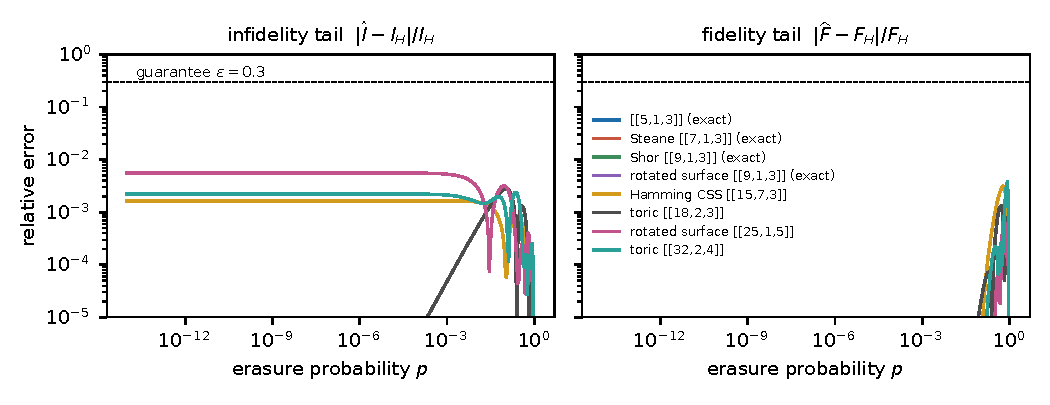
\includegraphics[width=\textwidth]{figures/validation.pdf}
\caption{Relative error of the output of the algorithm of
Theorem~\ref{thm:main}, run with off-the-shelf components, against the
exact curves, in both tails. The dashed line is the guaranteed
\(\eps\). Outputs that are exact do not appear on the logarithmic
scale.}
\label{fig:validation}
\end{figure}

Table~\ref{tab:computed-paper} and Figure~\ref{fig:validation} give the
result. The guarantee holds in both tails down to \(p=10^{-14}\), with
observed errors at most \(0.56\%\), a factor of more than fifty below
\(\eps\); the zero infidelity coefficients are reproduced exactly, so the
output has the right order of vanishing at \(p=0\); and on the four
smallest codes the whole output is exact. The cost is another matter.
The seven codes of at most 25 qubits took between less than a second and
23 minutes of single-thread time each. The 32-qubit toric code took 5.9
hours for its 66 counts, of which 2.7 went to three counts of the
\(\Bad\) formula, at \(j=9,10,11\). At a looser tolerance, single counts
on the 49- and 50-qubit codes took up to 161 seconds, against 39 seconds
at 32 qubits, and no count on the 72-qubit BB code completed within ten
minutes; we did not run the full algorithm beyond 32 qubits.
This is consistent with the purpose of Theorem~\ref{thm:main}, which is
a statement about exponents and not a recipe.

\subsection{A practical hybrid on the same certificate}
\label{sec:computed-hybrid}

For larger codes we use the SAT oracle only where sampling cannot work.
Call an erased set \emph{minimal uncorrectable} if \(d_E>0\) and every
proper subset is correctable. By inclusion monotonicity, a set is
uncorrectable exactly when it contains a minimal uncorrectable set.

\emph{Low layers.} A SAT solver enumerates \emph{all} minimal
uncorrectable sets of size \(1,2,\ldots,w\), level by level (in this
section \(w\) denotes this size bound and not an incidence count). The
formula
is the \(E\)-projection of the \(\Bad\) certificate in the form used for
Corollary~\ref{cor:uncorrectable}, except that the witness \(z\in N\) is
replaced by a fixed logical basis: there is \(x\in N\) supported on
\(E\) that anticommutes with some \(L_i\). At level \(w'\) we ask for
such a set of size at most \(w'\) that contains none of the sets found
so far, and add each answer as a blocking clause, until the instance is
unsatisfiable. Every answer \(E\) at level \(w'\) is minimal of size
exactly \(w'\): it contains a minimal uncorrectable set \(M\), and if
\(|M|<w'\) then \(M\) was found at an earlier, completed level and is
blocked, so \(|M|=w'\ge|E|\) and \(E=M\). The final unsatisfiable answer
says that the list is complete up to size \(w'\), and the first nonempty
level is the distance; these answers are checked independently below. For the toric and BB codes we use their
translation symmetry: every generating permutation is first checked to
preserve the row space of \(H\), so that the group they generate does,
each minimal set is added together with
its whole orbit, and the solver is asked only for sets through one
representative qubit of each orbit of qubits. This loses nothing: a
permutation that preserves \(S\) preserves \(d_E\) and maps minimal
uncorrectable sets to minimal uncorrectable sets, and every nonempty set
has a translate through a representative. For \(j\le w\) the layer sum
\(\sum_{|E|=j}(1-2^{-d_E})\) is supported on the union of the supersets
of the listed sets. We estimate it by the union estimator of Karp, Luby
and Madras~\cite{karplubymadras1989}: draw a listed set \(M\) with
probability proportional to its number of supersets of size \(j\), draw
a uniform superset \(E\supseteq M\) of size \(j\), compute \(d_E\) by
Gaussian elimination, and weight \(1-2^{-d_E}\) by the reciprocal of the
number \(\nu(E)\) of listed sets contained in \(E\). The estimator is
unbiased, and its relative variance is at most
\(\max_E\nu(E)\cdot g_{\max}/g_{\min}\), where \(g\) ranges over the
weights of uncorrectable sets (here \(g_{\max}/g_{\min}\le2\)); it does
not grow as uncorrectable sets become rare. Both facts are
machine-checked (\lean{UnionEstimator.mean\_sample},
\lean{UnionEstimator.second\_moment\_le}). We draw \(4\times10^5\)
union samples per layer (\(2\times10^5\) for the 128-qubit code). The
layer \(j=d\) is not
sampled at all: its uncorrectable sets are exactly the listed sets of
size \(d\), so the leading coefficient
\(\binom nd(1-f_d)=\sum_{|M|=d}(1-2^{-d_M})\) is a finite sum over the
list.

\emph{High layers.} The exponents of complementary sets satisfy
\(d_E+d_{E^{\mathrm c}}=2k\), so
\(f_j=4^{-k}\,\E_{|E'|=n-j}\bigl[2^{d_{E'}}\bigr]\), and
\(4^kf_j-1\) is again supported on uncorrectable sets, now of size
\(n-j\). For \(n-j\le w\) the same estimator applies with weight
\(2^{d_{E'}}-1\). Here \(g_{\max}/g_{\min}\) can be as large as
\(4^k-1\), but the estimated quantity \(x_j=4^kf_j-1\) enters
\(f_j=4^{-k}(1+x_j)\) only through \(1+x_j\), so a relative error in
\(x_j\) reaches \(f_j\) multiplied by \(x_j/(1+x_j)\).

\emph{Bulk.} For the remaining layers we sample \(2\times10^7\) erased
sets of size \(j\) uniformly and compute \(d_E\) for each. This suffices
when the relative standard errors of both \(f_j\) and \(1-f_j\) are at
most \(2\%\).

\emph{Layers just above \(w\).} Where it does not suffice, uncorrectable
sets are too rare to sample and too many to list. We split the layer
sum into the uncorrectable sets that contain a listed minimal set and
the remainder, those whose minimal subsets all have size above \(w\).
The first part is estimated by the union estimator, whose identity holds
for every \(j\). The remainder is sampled uniformly, and it is a small
part of the sum for \(j\) close to \(w\), so that an absolute error
which would be useless for the whole layer is enough for it. With \(M\)
samples we take its standard error to be at least \(3/M\), which is the
\(95\%\) upper bound on the remainder when no remainder event is seen.
The first sample is sized so that this floor meets the tolerance, and it
is doubled until the combined relative standard error is at most
\(2\%\).

The final coefficients are obtained from these estimates by the
repair~\eqref{eq:repair}, which by Lemma~\ref{lem:repair} preserves every
two-tail relative interval that the estimates satisfy coefficientwise.
Because both curves are positive combinations of the
coefficients, the relative error of \(\widehat I(p)\) and
\(\widehat F(p)\) at every \(p\) is at most the largest coefficientwise
relative error. The result is a statistical statement, with standard
errors from the central limit theorem for the unrepaired estimates, one
coefficient at a time and with no claim of simultaneous coverage, and
not the worst-case guarantee of Theorem~\ref{thm:main}. The
duality, the union identity and its split form, the minimal-set
characterization, the symmetry reduction and the passage from
coefficients to curves are machine-checked
(Table~\ref{tab:correspondence}); the sampling errors are not.

\emph{Proof-checked completeness.} The estimator needs three facts about
a list: every listed set is uncorrectable, none is smaller than \(d\),
and every uncorrectable set of size at most \(w\) contains a listed set.
The first two are checked by Gaussian elimination. For the third we
rely neither on the solver that produced the list nor on a program that
writes its input. The statement ``there is an uncorrectable set of size
at most \(w'\) that contains no listed set'' is a CNF formula defined in
Lean (\lean{certFormula}), with a proof that its unsatisfiability gives
the completeness of the list through \(w'\)
(\lean{certFormula\_unsat}). A Lean program writes the formula,
CaDiCaL~\cite{biere2024cadical} refutes it and emits a proof in the LRAT
format~\cite{cruzfilipe2017lrat}, and the same program checks that proof
with the LRAT checker of the Lean~4 core library, whose soundness is a
theorem of that library (\lean{LRAT.check\_sound}). The symmetry
reduction, and a case split of the instances whose proofs are too large
to check in memory, are covered by the theorem. A second Lean program,
whose checks are proved sound, verifies the side conditions, and one
theorem (\lean{ListCertificate.symmetric\_certificate}) then gives the
completeness of the list through \(w'\), the distance, the
identification of the uncorrectable sets of size \(d\) with the listed
ones, and the exact leading layer sum.
For nine of the ten codes every level up to \(w\) is verified in this way. For the \([[128,2,8]]\) code the levels through size 12 of 15 are, which covers its distance, its sets of size \(d\) and its leading layer sum; sizes 13 to 15 were beyond our computing budget with this formula and are certified with an independently written encoding, whose refutations are proof-checked in the same way but whose meaning is tested against exhaustive enumeration on small codes and not proved.
What remains trusted is the parser of the certificate file, the compiled
code of the Lean functions and the matching, by SHA-256 hash, of the
instances whose proofs were checked with those used in the final
combination.


We checked the estimator against exhaustive enumeration on the
\([[18,2,3]]\), \([[25,1,5]]\) and \([[32,2,4]]\) codes, the last over
all \(2^{32}\) erased sets. The repaired curves of the runs reported
below differ from the exact ones by at most \(1.4\times10^{-4}\) in
relative terms, in either tail, over the same grid of \(p\) as in
Table~\ref{tab:computed-paper}. In separate validation runs with
\(4\times10^6\) uniform samples per bulk layer, no layer estimate of any
kind deviates from the exact coefficient by more than \(2.4\) reported
standard errors. These runs never need the split estimator. To exercise
it we reran the \([[25,1,5]]\) and \([[32,2,4]]\) codes with \(w=d\) and
only \(2\times10^4\) uniform samples per layer, which forces the
split on three and five layers; all sixteen split estimates of
\(1-f_j\) and of the uncorrectable fraction are within two standard
errors of the exact values.

\begin{table}[htbp]
\centering\small
\setlength{\tabcolsep}{4pt}
\begin{tabular}{@{}lp{0.26\textwidth}rrrrrr@{}}
\toprule
Code & minimal uncorrectable sets, size:\,count & $w$ & s.e. & $I_H(10^{-3})$ & $I_H(10^{-2})$ & $I_H(0.1)$ & $p_{1/2}$\\
\midrule
toric $[[18,2,3]]$ & 3:\,12, 5:\,72, 6:\,78 & 6 & 0.02\% & $6.0\times10^{-9}$ & $6.0\times10^{-6}$ & $0.00626$ & 0.443\\
surface $[[25,1,5]]$ & 5:\,104, 7:\,150 & 8 & 0.05\% & $5.2\times10^{-14}$ & $5.2\times10^{-9}$ & $4.7\times10^{-4}$ & 0.538\\
toric $[[32,2,4]]$ & 4:\,16, 6:\,192, 8:\,1064, 10:\,3136 & 10 & 0.04\% & $8.0\times10^{-12}$ & $8.0\times10^{-8}$ & $8.9\times10^{-4}$ & 0.456\\
surface $[[49,1,7]]$ & 7:\,592, 9:\,1954, 11:\,4548, 13:\,8076 & 13 & 0.2\% & $3.0\times10^{-19}$ & $2.9\times10^{-12}$ & $2.7\times10^{-5}$ & 0.530\\
toric $[[50,2,5]]$ & 5:\,20, 7:\,400, 9:\,2200, 10:\,2410, 11:\,8000 & 11 & 0.2\% & $1.0\times10^{-14}$ & $1.0\times10^{-9}$ & $1.2\times10^{-4}$ & 0.463\\
BB $[[72,12,6]]$ & 6:\,156, 8:\,1980, 10:\,26496 & 11 & 0.7\% & $8.1\times10^{-17}$ & $8.1\times10^{-11}$ & $9.2\times10^{-5}$ & 0.373\\
toric $[[72,2,6]]$ & 6:\,24, 8:\,720, 10:\,5760, 12:\,37572 & 13 & 0.9\% & $1.2\times10^{-17}$ & $1.2\times10^{-11}$ & $1.6\times10^{-5}$ & 0.467\\
surface $[[81,1,9]]$ & 9:\,3112, 11:\,16542, 13:\,61350 & 14 & 2.0\% & $1.6\times10^{-24}$ & $1.5\times10^{-15}$ & $1.4\times10^{-6}$ & 0.525\\
BB $[[90,8,10]]$ & 10:\,1116, 12:\,20580 & 13 & 1.9\% & $5.6\times10^{-28}$ & $5.6\times10^{-18}$ & $6.7\times10^{-8}$ & 0.431\\
toric $[[128,2,8]]$ & 8:\,32, 10:\,1792, 12:\,25984, 14:\,195328 & 15 & 2.0\% & $1.6\times10^{-23}$ & $1.6\times10^{-15}$ & $2.6\times10^{-7}$ & 0.473\\
\bottomrule
\end{tabular}

\caption{The hybrid estimator. ``Minimal uncorrectable sets'' lists the
number found at each size up to the level \(w\) through which the SAT
enumeration is complete; sizes not listed have none, and the first size
is the distance \(d\). ``s.e.''\ is the largest relative standard error
over all coefficients of either tail, which bounds the relative standard
error of both curves at every \(p\); in the split layers it includes the
\(3/M\) convention described in the text. \(p_{1/2}\) is the erasure
probability at which \(I_H(p)=1/2\).}
\label{tab:computed-hybrid}
\end{table}

\begin{figure}[htbp]
\centering
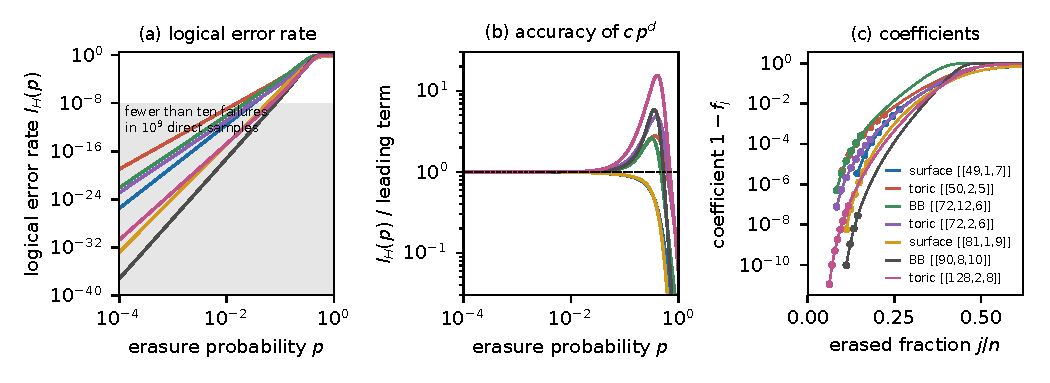
\includegraphics[width=\textwidth]{figures/curves.pdf}
\caption{(a) The logical error rate \(I_H(p)\) of the optimal erasure
decoder for the seven largest codes of Table~\ref{tab:computed-hybrid}.
In the shaded region a direct simulation with \(10^9\) samples expects
fewer than ten failures. (b) The ratio of \(I_H(p)\) to its leading term
\(\binom nd(1-f_d)\,p^d\). (c) The infidelity coefficients \(1-f_j\);
dots mark the layers \(j\le w\), which are computed from the
SAT-enumerated minimal sets alone.}
\label{fig:curves}
\end{figure}

Table~\ref{tab:computed-hybrid} and Figure~\ref{fig:curves} give the
results for ten codes of 18 to 128 qubits. The SAT enumeration took at
most three minutes for each of the eight codes of at most 81 qubits, 43
minutes for the \([[90,8,10]]\) code and 13 minutes for the
\([[128,2,8]]\) toric code, on up to twelve solver threads; the sampling took between 23
seconds and about 110 minutes per code on 8 to 24 threads. The split
estimator was needed on one layer of the \([[81,1,9]]\) code, on eight
layers (\(j=14,\ldots,21\)) of the \([[90,8,10]]\) code and on eleven
(\(j=16,\ldots,26\)) of the \([[128,2,8]]\) code, with up to \(1.6\times10^9\)
samples in a layer; the sampled remainder was at most \(3\%\) of a layer
sum. Every coefficient of every code has a relative standard error of at
most \(2\%\) on both scales; in the fourteen of the twenty split
layers where no remainder event was seen, the error assigned to the
remainder is the \(95\%\) bound \(3/M\). Three observations follow.

\emph{Small \(p\).} At \(p=10^{-3}\) the logical error rate ranges from
\(6\times10^{-9}\) for the smallest code to \(5.6\times10^{-28}\) for the
\([[90,8,10]]\) code, and at \(p=10^{-2}\) it is below \(10^{-10}\) for
six of the ten codes. No direct Monte Carlo simulation reaches these
values; here they come with the same relative error as the rest of the
curve, because the low layers are computed from the enumerated sets. The
first nonempty level reproduces the distance of every code, and the
leading coefficient \(c=\binom nd(1-f_d)\) is exact, with the
completeness of the list of minimum-size sets proof-checked as described
above: \(c=2L\) for the
\(L\times L\) toric code, whose \(4L\) uncorrectable sets of size \(L\)
all have \(d_E=1\); \(c=52\), \(296\) and \(1556\) for the surface codes
of distance \(5\), \(7\) and \(9\); \(c=81\) for the \([[72,12,6]]\) code,
which has 144 uncorrectable sets of size six with \(d_E=1\) and 12 with
\(d_E=2\); and \(c=558\) for the \([[90,8,10]]\) code.

\emph{The leading term.} As \(p\to0\) the curve approaches its leading
term \(c\,p^d\). Figure~\ref{fig:curves}(b) shows, for the seven largest
codes, how soon the two separate. At \(p=0.05\) the ratio \(I_H(p)/(c\,p^d)\) is within
\(8\%\) of one for nine codes and is \(1.14\) for the 128-qubit toric
code. At \(p=0.1\) it is between \(1.14\) and \(1.30\) for the toric and
BB codes of 50 to 90 qubits and \(1.61\) for the 128-qubit toric code,
and it peaks between \(p=0.31\) and \(p=0.41\) at \(2.6\), \(2.8\),
\(4.8\), \(5.9\) and \(15.6\) for the \([[72,12,6]]\), \([[50,2,5]]\),
\([[72,2,6]]\), \([[90,8,10]]\) and \([[128,2,8]]\) codes. For the
surface codes the deviation has the other sign: the ratio is about
\(0.91\) at \(p=0.1\) and about \(0.6\) at \(p=0.3\). The distance and the
number of minimum-size uncorrectable sets therefore do not give the
logical error rate at erasure probabilities of about ten percent and
above, and the direction of the error depends on the code family; the graded
coefficients of Figure~\ref{fig:curves}(c) are what is needed.

\emph{The transition.} The erasure probability \(p_{1/2}\) at which
\(I_H=1/2\) increases with the size of the toric
code (\(0.443\), \(0.456\), \(0.463\), \(0.467\), \(0.473\) for
\(L=3,4,5,6,8\)) and decreases with the size of the surface code
(\(0.538\), \(0.530\), \(0.525\)), which is consistent with the erasure
threshold \(1/2\) of these families~\cite{stace2009}. The two BB codes,
which encode twelve and eight qubits, have \(p_{1/2}=0.373\) and
\(0.431\); since \(I_H\) saturates at \(1-4^{-k}\), these values should
not be compared across different \(k\).

\subsection{Limits}
\label{sec:computed-limits}

The algorithm of Theorem~\ref{thm:main}, run with an off-the-shelf
hashing counter, reached 32 qubits on a workstation. Its guarantee held
with a wide margin wherever it could be checked, so the limit is cost;
we made no attempt to tune the counter or the encoding. The hybrid
estimator is limited by the unsatisfiable instance that closes a level,
which becomes harder with the level and with the distance (we did not
attempt the \([[144,12,12]]\) BB code), and by the size of the lists,
195{,}328 sets of size 14 for the 128-qubit code. In the layers between
\(w\) and those where uncorrectable sets are common, the remainder is
known only from uniform sampling. It cannot be missed silently, since it
is sampled from the whole layer, but if \(w\) were further from the
sampled layers it would dominate and the method would report a large
error. The estimates are statistical; what is proof-checked is the
completeness of the lists, with the exception stated above for the
largest code. The layer structure used here is that of the iid channel,
and we did not implement the multiclass or latent-circuit versions.

\section{Correlated erasures generated by a latent circuit}
\label{sec:latent}

The same reduction applies to a specified class of correlated erasures.
Let \(C:\{0,1\}^r\to\{0,1\}^n\) be a supplied deterministic circuit
over a fixed bounded-arity Boolean basis, independent of the probability
parameters. Count both gates and wires, including output wires, in \(s_C\).
Draw the latent bits independently with common probability \(p\), set
\(E=C(b)\), and apply ordinary erasure of \(E\) to the encoded state.
The draw is independent of that state. Recovery receives the exact set
\(E\), but not \(b\). Write \(F_{H,C}(p)\) for optimal
entanglement fidelity of the maximally mixed logical input, and
\(I_{H,C}(p)=1-F_{H,C}(p)\).

\begin{theorem}[Latent-circuit transfer]\label{thm:latent}
Assume the SAT algorithm of Theorem~\ref{thm:main}. Put
\[
 V=n+r+w+s_C,\qquad q=r+2n,\qquad
 L=n+r+\operatorname{len}(H,C,\eps,\delta),
\]
where \(w=\operatorname{nnz}(H)\) and \(\operatorname{len}\) denotes
the sum of encoding lengths. For \(r\ge1\), a randomized algorithm
returns rational coefficients \(\widehat f_0,\ldots,\widehat f_r\).
Define
\[
 \widehat F(p)=\sum_{j=0}^r\widehat f_j\binom rj p^j(1-p)^{r-j},
 \qquad \widehat I(p)=1-\widehat F(p).
\]
With probability at least \(1-\delta\), simultaneously for all
\(p\in[0,1]\),
\[
 |\widehat F(p)-F_{H,C}(p)|\le\eps F_{H,C}(p),\qquad
 |\widehat I(p)-I_{H,C}(p)|\le\eps I_{H,C}(p).
\]
Every run has \(0\le\widehat f_j\le1\), exact zero infidelity
coefficients, and exact endpoints
\[
 \widehat f_0=2^{-d_{C(0^r)}},\qquad
 \widehat f_r=2^{-d_{C(1^r)}}.
\]
If \(C\) is promised coordinatewise monotone, the coefficients can
also be chosen nonincreasing, so \(\widehat F\) is nonincreasing
and \(\widehat I\) is nondecreasing. No monotonicity is asserted
for a general circuit.

The algorithm uses polynomial space and
\[
 O\!\left((r+1)(q+1)^2\eps^{-2}
       \log\frac{2(r+1)}{\delta}\right)
\]
SAT calls, each with \(O(V)\) variables and clauses of width at most
three. Its time is
\[
 \poly(L,\eps^{-1},\log\delta^{-1})T(KV)
\]
for a constant \(K\) that depends only on the gate basis, and each
coefficient has
\(O(n+r+\log\eps^{-1})\) bits.
For \(r=0\), one fixed erased set is evaluated exactly by binary
linear algebra.
\end{theorem}

\begin{proof}
All latent causes with the same \(E\) induce the same erasure channel,
so one optimal recovery for the revealed \(E\) serves every such cause,
and Lemma~\ref{lem:fidelity} gives
\[
 F_{H,C}(p)=\sum_{b\in\{0,1\}^r}
       p^{|b|}(1-p)^{r-|b|}\,2^{-d_{C(b)}}.
\]
For each \(j\), let \(A_j^C\) and \(B_j^C\) be the numbers of pairs
\((b,z)\) with \(|b|=j\) and \(z\in N\) that satisfy \(\Good(C(b),z)\)
and \(\Bad(C(b),z)\), respectively. Append full-equivalence Tseitin
clauses for \(C\) to the certificate circuits of Lemma~\ref{lem:cnf},
with a population counter for \(|b|=j\), and project onto \((b,z)\)
only; this uses \(O(V)\) variables and clauses. The projection must be
onto \(b\) and not onto \(E\), because different \(b\) with the same
\(E\) carry probabilities that must be added.
Proposition~\ref{prop:cert} gives \(A_j^C+B_j^C=\binom rjZ\) and
\(f_j^C=A_j^C/(\binom rjZ)\).

The rest follows the proof of Theorem~\ref{thm:main}, with \(q=r+2n\)
projection bits and \(2(r+1)\) counts: estimate, normalize, and replace
the two endpoint coefficients by their exact values, computed by linear
algebra. For an arbitrary circuit these coefficients are the output,
without shape repair; positivity of the Bernstein weights gives both
relative guarantees, and the SAT zero tests retain every zero infidelity
coefficient, whether or not the zero layers form an initial segment.
Under the monotonicity promise, \(b\le b'\) implies
\(C(b)\subseteq C(b')\) and \(d_{C(b)}\le d_{C(b')}\), so
\(f_0^C\ge\cdots\ge f_r^C\) by the same coupling, and
Lemma~\ref{lem:repair} with anchors \(\{0,r\}\) gives the shape. In that
case the zero infidelity layers are exactly \(j<d_C\), where
\(d_C=\min\{|b|:d_{C(b)}>0\}\) (infinite if no latent assignment is
uncorrectable) is a latent fault weight, not the code distance.
\end{proof}

If \(r,w,s_C=O(n)\), the instantiation of
Corollary~\ref{cor:unconditional} again gives the
rate~\eqref{eq:formalrate}, and Remark~\ref{rem:sharp} the
rate~\eqref{eq:sharp} under its hypothesis.

Monotonicity genuinely needs an additional hypothesis. For one
unencoded qubit and \(C(b_1,b_2)=b_1\mathbin{\mathrm{XOR}}b_2\),
the exact fidelity coefficients are \((1,1/4,1)\), and
\[
 I_{H,C}(p)=\tfrac32p(1-p).
\]
The endpoint fidelities are both one, although the interior
infidelity is positive.

\subsection{A fixed number of latent probability classes}
\label{sec:multiclass}

Partition the latent bits into a fixed number \(t\) of classes
of sizes \(r_1,\ldots,r_t\), with independent bits of probability
\(p_a\) in class \(a\), and \(\sum_a r_a=r\).
Include the partition description in \(L\).
For a weight vector \(\mathbf j=(j_1,\ldots,j_t)\) with
\(0\le j_a\le r_a\), define \(A_{\mathbf j}^C\)
and \(B_{\mathbf j}^C\) by the same projected certificates,
requiring weight \(j_a\) in each class. Then
\[
 A_{\mathbf j}^C+B_{\mathbf j}^C
   =Z\prod_{a=1}^t\binom{r_a}{j_a},\qquad
 f_{\mathbf j}^C=
 \frac{A_{\mathbf j}^C}{Z\prod_a\binom{r_a}{j_a}},
\]
and
\[
 F_{H,C}(\mathbf p)=
 \sum_{\mathbf j} f_{\mathbf j}^C
 \prod_{a=1}^t\binom{r_a}{j_a}p_a^{j_a}(1-p_a)^{r_a-j_a}.
\]
There are \(Q=\prod_a(r_a+1)\le(r+1)^t\) coefficients. Order the index
set \(J=\prod_a\{0,\ldots,r_a\}\) componentwise, and call
\(\mathbf j\) a \emph{corner} if each \(j_a\in\{0,r_a\}\); there are at
most \(2^t\) distinct corners, fewer when some \(r_a=0\).

\begin{theorem}[Multiclass transfer with exact-corner tensor repair]
\label{thm:multiclass}
Assume the SAT algorithm of Theorem~\ref{thm:main}, and fix \(t\).
There is a randomized algorithm that, given \(H\), \(C\), the class
partition and rational \(0<\eps,\delta<1\), returns rational
coefficients \((\widehat f_{\mathbf j})_{\mathbf j\in J}\) in \([0,1]\)
such that, with
\(\widehat F(\mathbf p)=\sum_{\mathbf j}\widehat f_{\mathbf j}
 \prod_a\binom{r_a}{j_a}p_a^{j_a}(1-p_a)^{r_a-j_a}\)
and \(\widehat I=1-\widehat F\), with probability at least \(1-\delta\),
simultaneously for every \(\mathbf p\in[0,1]^t\),
\[
 |\widehat F(\mathbf p)-F_{H,C}(\mathbf p)|\le\eps F_{H,C}(\mathbf p),
 \qquad
 |\widehat I(\mathbf p)-I_{H,C}(\mathbf p)|\le\eps I_{H,C}(\mathbf p).
\]
On every run, \(\widehat F+\widehat I=1\), both curves take values in
\([0,1]\), zero infidelity coefficients are retained exactly, and every
corner coefficient equals the exact fidelity
\(2^{-d_{C(b_{\mathbf j})}}\) of the single latent assignment
\(b_{\mathbf j}\) in that layer. If \(C\) is coordinatewise monotone, the
table \(\widehat f\) is antitone in the componentwise order on every run,
so \(\widehat F\) is nonincreasing and \(\widehat I\) nondecreasing in
each \(p_a\).
The algorithm makes
\[
 O\!\left(Q(q+1)^2\eps^{-2}\log\frac{2Q}{\delta}\right)
\]
SAT calls with \(q=r+2n\), each with \(O(V)\) variables and clauses of
width at most three, and runs in time
\(\poly(L,Q,\eps^{-1},\log\delta^{-1})\,T(KV)\) and space
\(\poly(L,Q)\). The output has \(Q\) coefficients of
\(O(n+r+\log\eps^{-1})\) bits each.
\end{theorem}

The dependence on \(Q\) is stated explicitly: for fixed \(t\) it is
polynomial in \(r\), and no polynomial output bound is claimed for a
separate probability for every bit.

\begin{proof}
The classwise population counters have total size \(O(r)\), so the
projected counting instances remain of size \(O(V)\). Apply
Proposition~\ref{prop:counter} to both counts in every layer with
tolerance \(\eps/3\) and failure probability \(\delta/(2Q)\), and
normalize as in Theorem~\ref{thm:latent}; on a single event of
probability at least \(1-\delta\) every \(g_{\mathbf j}\) lies in its
two-tail interval, and the tensor-Bernstein weights are nonnegative and
sum to one. Each corner layer contains a single latent assignment, whose
fidelity is computed exactly by linear algebra and substituted. For a
general circuit this table is the output; whether the repair below is
applied is part of the input, since monotonicity of \(C\) is not tested.

When \(C\) is coordinatewise monotone the true table is antitone: for
\(\mathbf j\le\mathbf j'\), extend within each class a uniform
weight-\(j_a\) set to a uniform weight-\(j'_a\) superset; then
\(C(b)\subseteq C(b')\) and \(f_{\mathbf j}\ge f_{\mathbf j'}\). Apply
Lemma~\ref{lem:repair} on \((J,\le)\) with the corners as anchors and
the endpoints~\eqref{eq:twotail}. The output is antitone on every run,
exact at the corners, and accurate on the accuracy event, and
\(\partial_{p_a}\widehat F\le0\) by the one-variable Bernstein
derivative. The repair makes \(O(Q^2)\) comparisons of stored ratios,
the oracle budget is \(2Q\) applications of
Proposition~\ref{prop:counter}, and neither \(Q\) nor the accuracy
parameters enter the argument of \(T\).
\end{proof}

Theorem~\ref{thm:multiclass} with \(t=1\), \(r=n\) and \(C\) the identity
recovers the iid curve of Theorem~\ref{thm:main}. The machine-checked
form of Theorem~\ref{thm:main} is proved as exactly this specialization
and then restated for the iid channel without tensor vocabulary
(Section~\ref{sec:formal}).

\paragraph{Examples.}
For independently triggered loss events with supports \(D_\gamma\),
\(E_i=\bigvee_{\gamma:\,i\in D_\gamma}b_\gamma\) is monotone even when
supports overlap, and has linear circuit size when \(r=O(n)\) and
\(\sum_\gamma|D_\gamma|=O(n)\); this includes a constant-length burst
triggered at each starting position. A second example is the
deterministic-emission Gilbert--Elliott erasure
model~\cite[Section VI]{adlercassuto2017} with a fixed initial state:
\(S_i=(\neg S_{i-1}\wedge A_i)\vee(S_{i-1}\wedge D_i)\) and \(E_i=S_i\),
with independent \(A_i,D_i\) of probabilities \(\alpha,1-\beta\), is an
\(O(n)\)-size circuit with two probability classes. It is not monotone,
so the accuracy guarantee applies without the shape. Correlated
gate-associated atom
loss~\cite{perrinloss2026,perrin2025atomloss,baranes2026loss} motivates
such models; the extension covers loss patterns that are sampled
independently of the encoded state and revealed exactly to the recovery,
not state-dependent loss or noisy circuit dynamics.

\section{Formal verification}
\label{sec:formal}

The reduction of this paper has been formalized in Lean~4 as a concrete
machine, and composed with a verified external SAT engine. This section
states exactly what has been checked, in which toolchain, and what has
not. All checked statements depend only on Lean's standard axioms
\lean{propext}, \lean{Classical.choice} and \lean{Quot.sound}, as
reported by \lean{\#print axioms} for each named theorem; no
\lean{sorry}, added \lean{axiom} or \lean{native\_decide} occurs.

\subsection{The checked statements}

\paragraph{The composition with a verified engine.}
Under Lean v4.34.1 and Mathlib commit \texttt{d13f23b7}, the external
development of~\cite{openai2026eth} (commit \texttt{4eaee875}, with
proof-internal and import-only edits to 108 of its files that leave
every exported statement unchanged and are listed in the artifact) and
the reduction
are checked in one 6{,}157-module graph. The engine is consumed through
its theorem \lean{SqrtLogSpace.sat\_polynomial\_space}, described in the
proof of Corollary~\ref{cor:unconditional}. The reduction is stated
against a contract for a SAT machine, \lean{ResourceEncodedSAT}, which
charges the ambient variable count in unary plus the binary query
length, and the bridge theorem
\lean{ConcreteSolver.exists\_resource\_machine} proves that one fixed
engine satisfies it (for requests with at most as many clauses as
variables; the reduction pads its queries to meet this), with polynomial
envelopes and the monotone runtime envelope
\(T(v)=\max_{s\le v}\lceil2^{A\rho(s)}\rceil+1\). Its proof uses the
verified encoding bridge, the satisfiability-preserving formula
translation and a proved polynomial bound on the frontend's own time and
space. The closed theorems below therefore have no SAT, hashing,
certificate or physical-lift hypothesis. The same guarantee for an
arbitrary engine that satisfies the contract, with \(T\) as a
parameter and with the hash certificate and the physical lift as
hypotheses, is \lean{TensorMachine.Runtime.tensor\_machine\_guarantee},
stated for probability classes.

\paragraph{Theorem~\ref{thm:main} and Corollary~\ref{cor:unconditional}
as one declaration.}
The theorem
\begin{center}
\lean{QecReliability.IidErasure.iid\_erasure\_machine\_guarantee}
\end{center}
states the iid case directly: the channel, the coefficients and the
guarantee are expressed without latent circuits or tensor vocabulary.
There exist an engine, a rate constant \(A>0\) and polynomial envelopes
\(P_t,P_s\) such that, for every \(n\), every list of check rows on \(n\)
qubits with isotropic row space \(S\), and all natural numbers
\(0<a\le b\), \(0<c\), \(0<d\) (so \(\eps=a/b\), \(\delta=c/d\)):
\begin{enumerate}
\item[(i)] the entanglement fidelity \(F(p)\) of one fixed flag decoder
 composed with the channel that erases each qubit independently with
 probability \(p\) equals \(\sum_jf_j\Bern nj\), where \(f_j\) is the
 average of \(2^{-d_E}\) over \(|E|=j\), and no recovery channel has
 larger fidelity, for every \(p\in[0,1]\);
\item[(ii)] for \emph{every} string of \(N\) coin bits appended to the
 input, the fixed machine \(M\) has a completed run that leaves a
 rational vector \((\widehat f_0,\ldots,\widehat f_n)\) on its output
 tape, in time at most \(P_t(L_*)(B+1)\bigl(T(\kappa'(L_{\mathrm{code}}+1))+1\bigr)\)
 and at most \(P_s(L_*)\) visited cells, with
 \(1=\widehat f_0\ge\widehat f_1\ge\cdots\ge\widehat f_n=F(1)=4^{-(n-\dim S)}\)
 and \(\widehat f_j=1\) if and only if \(f_j=1\);
\item[(iii)] with probability at least \(1-c/d\) over the uniform law on
 the \(N\) coins, the curve
 \(\widehat F(p)=\sum_j\widehat f_j\Bern nj\) satisfies
 \(|\widehat F(p)-F(p)|\le\eps F(p)\) and
 \(|\widehat F(p)-F(p)|\le\eps(1-F(p))\) simultaneously for every
 \(p\in[0,1]\).
\end{enumerate}
Here \(N\) is a number of coin bits and not the normalizer,
\(T(v)=\max_{s\le v}\lceil2^{A\rho(s)}\rceil+1\),
\(B=\lceil144b^2/a^2\rceil\), \(\kappa'\) is a fixed constant,
\(L_{\mathrm{code}}=2n+\mathrm{nnz}(H)+1\), and \(L_*=L+t+Q\) in the
notation of Theorems~\ref{thm:latent} and~\ref{thm:multiclass}, with one
class of size \(n\) (\(t=1\), \(Q=n+1\)) and the identity circuit.
Item~(ii) is the monotone shape, the exact endpoints and the
deterministic identification of zero infidelity coefficients of
Theorem~\ref{thm:main}, for the coefficients the machine writes. The
statement differs from the prose of Theorem~\ref{thm:main} in three
ways. It makes no sparsity assumption, and the argument of \(T\) is
linear in \(n+\mathrm{nnz}(H)\), where \(\mathrm{nnz}(H)\) stands for the
total length of the coordinate lists that present the rows. The
confidence parameter enters the time and space bounds only through
\(L_*\), which includes the encodings of \(c\) and \(d\). And the
machine is the multiclass machine, run on one class and an encoding of
the identity circuit; the theorem is proved by this specialization and a
proved identity between the one-class tensor channel and the iid
channel.

\paragraph{Resources and the other closed theorems.}
A second form of the theorem,
\begin{center}
\lean{IidErasure.iid\_erasure\_machine\_guarantee\_resources},
\end{center}
adds the
content of Proposition~\ref{prop:resources} with explicit constants, for
every coin string: each output coefficient is a pair of natural numbers
of at most \(3n+\lceil\log_2(4B+1)\rceil+1\) bits; the counting
procedure makes at most \(512(L_*+1)^4(B+1)\) SAT calls; and every query
is a width-three request with at most \(\kappa'(L_{\mathrm{code}}+1)\)
variables and as many clauses. The calls counted are those of the
source-level counting procedure whose output the machine writes; they
are tied to the machine run through the time bound, and not by an
identification with tape-level engine invocations.

The other models have closed theorems of the same form
(Table~\ref{tab:correspondence}):
\begin{center}\small
\begin{tabular}{@{}p{0.56\textwidth}p{0.40\textwidth}@{}}
\toprule
Declaration & Model\\
\midrule
\lean{isotropic\_polynomial\_endpoint\_machine\_guarantee} &
latent circuit, arbitrary (Theorem~\ref{thm:latent})\\
\lean{latent\_monotone\_machine\_guarantee} &
latent circuit, monotone\\
\lean{isotropic\_tensor\_machine\_guarantee\_strong} &
probability classes, monotone (Theorem~\ref{thm:multiclass})\\
\lean{isotropic\_tensor\_machine\_guarantee\_general} &
probability classes, arbitrary\\
\lean{uncorrectable\_machine\_guarantee\_sized} &
\(U_H\), through the repeated code of
Remark~\ref{rem:uncorrectable-machine}\\
\bottomrule
\end{tabular}
\end{center}
In every one of them the engine, the rate constant and the polynomial
envelopes are chosen \emph{before} the dimensions and inputs, and the
machine depends only on the engine and a fixed program. The theorem for
an arbitrary latent circuit has no monotone-shape conclusion, because
its machine applies no repair; below it is called the latent theorem,
and the theorem for monotone probability classes the strengthened
multiclass theorem. All statements, and that of the external
engine, are reproduced verbatim in the artifact's \texttt{docs/} folder,
with the audit files in \texttt{tools/audit/}; their
full text is longer than a page because every bound is written out.

Two audits of the compiled graph, one printing the axioms of the 147
declarations cited in this section and in
Table~\ref{tab:correspondence} by name, the other collecting the axioms
of all 2{,}386 declarations of the thirty-four final modules, report
only the three standard axioms.

\subsection{Correspondence with the paper}

Kernel checking establishes the Lean statements, not their identity with
the prose. Table~\ref{tab:correspondence} in
Appendix~\ref{app:correspondence} records the correspondence claim by
claim. In summary: every theorem, proposition, corollary and lemma of
Sections~\ref{sec:results}--\ref{sec:latent} has a kernel-checked
counterpart, at machine level for the algorithmic statements, with four
exceptions that are stated there: the rates of
Remarks~\ref{rem:sharp} and~\ref{rem:anthropic}, the final step to
NP-hardness, where the reduction from SAT is checked but the
Cook--Levin theorem and the polynomial running time of the reduction
are not,
the explicit hash of Appendix~\ref{app:hash}, for which the machines use
a different certificate, and the direct algorithm in the proof of
Corollary~\ref{cor:uncorrectable}, which is checked at the level of its
formula while the machine-level theorem runs a different algorithm. The exact-distance and weight-enumerator algorithms of
Section~\ref{sec:hardness}, which are not numbered statements, are
checked at the level of their formulas only. The numerical content of
Section~\ref{sec:computed} is experimental, with two exceptions described
there: the exhaustive tables of the seven codes of at most 25 qubits
were recomputed by a verified Lean function, and the lists of minimal
uncorrectable sets are certified complete. These certificates are
results of running compiled Lean programs whose checks are proved
sound; they are not theorems reduced in the kernel.

\subsection{Trusted base, constants, and artifact}

The trusted base is the Lean~4 kernel, Mathlib, and the definitions on
both sides of the bridge: the external development's CNF semantics,
machine model and input encoding, and our definitions of the erasure
channel, entanglement fidelity, the multitape machine, completed runs,
visited cells and the output predicate. The machine model is a
deterministic finite-state multitape machine; the external
\lean{PrimitiveMachine} scans one cell per step and is transported into
it with a proved time and space overhead. Two kinds of non-transparent
declaration occur and introduce no axiom: the external solver seals six
finite instruction tables as \lean{private opaque} constants, and our
tactic support code contains three \lean{partial def} helpers. An independent kernel replay
with \texttt{leanchecker}, which re-checks every declaration of a module
in the kernel from its compiled imports, was run on all 6{,}157 modules
of the graph, Mathlib and the external solver included, and passed.

Every closed statement is existential in the engine, the rate constant
and the polynomial envelopes, and the reliability program depends on a
fixed hash certificate. The constants are doubly exponential: the
certificate's expander walk has \(2^{56}\) steps, so the random-bit
length \(N\) and the SAT-size constant \(\kappa\) both exceed
\(2^{2^{58}}\) for every input, including \(n=0\). The theorems are
therefore asymptotic statements, as Remark~\ref{rem:crossover} says for
the paper constants.

The Lean development, the audit files, and the code and data of the
experiments are public at
\url{https://github.com/Oliverds321/stabilizer-erasure-sat-lean}; this paper
describes release \texttt{v1.0.0}.

\section{Related work}
\label{sec:related}

\paragraph{Erasure in quantum codes.}
The quantum erasure channel and its capacity are classical
topics~\cite{grassl1997,bds1997}. The per-pattern optimum \(2^{-d_E}\),
the rank-of-\(H_E\) combinatorics and equal coset probabilities appear in
Delfosse and Zémor's rate bounds for LDPC stabilizer
codes~\cite{delfossezemor2013}, in the optimal recovery probability of
Gullans et al.~\cite{gullans2021}, and in degenerate erasure
decoding~\cite{kuoouyang2026}. Fast maximum-likelihood erasure decoders
exist for surface and hypergraph-product
codes~\cite{delfossezemor2020,connolly2024}. Ashikhmin~\cite{ashikhmin2020}
studies finite-length codes on the same channel. That paper states the
recoverability criterion, the per-pattern fidelity and the comparison
\(I_H\le U_H\le2I_H\), and then bounds the probability \(P_{de}\) of an
unrecoverable pattern, our \(U_H\), over all codes of given parameters,
by MacWilliams-type identities, linear programming and random-coding
arguments; it does not consider computing the curve of a given code.
Our enumeration reproduces the seventeen invariants printed in its
Example~1, and the verified table of \lean{ExactTable} its numbers of
unrecoverable sets (script \texttt{ashikhmin\_example.py}).
Mandal, Gökduman and Pfister~\cite{mandal2026area} prove area theorems
and an erasure-folding identity for a related but different curve, the
entropy of the logical correction class given the syndrome, which for
erasure is linear in \(d_E\) where ours is \(2^{-d_E}\); the expression of
erasure failure as a sum over uncorrectable patterns is used in Freire
et al.~\cite{freire2026maxwell}.
Rare-event estimation of logical error rates by splitting and subset
sampling~\cite{bravyivargo2013,heussen2024subset,mayer2026rare,beverland2025},
coherent-information thresholds by Monte Carlo over erasure
configurations~\cite{colmenarez2025}, statistical-mechanics estimates of
logical error curves under Pauli noise~\cite{wichette2026}, and shot-free
leading-order predictors~\cite{sethi2026} are the practical
alternatives; none gives a worst-case relative guarantee on the whole
curve. The hybrid estimator of Section~\ref{sec:computed-hybrid} belongs
with these methods: it stratifies by erasure weight, as subset sampling
does, and replaces sampling in the rare layers by a complete SAT
enumeration of minimal uncorrectable sets.

\paragraph{Enumerators and hardness in quantum coding.}
Quantum weight enumerators~\cite{shorlaflamme1997,rains1998} and their
tensor-network generalizations~\cite{caolackey2022,cao2024expansion}
compute exact logical error rates when a low-complexity contraction
exists; support-sensitive enumerators~\cite{scott2005} contain erasure
information. Decoding stabilizer codes is NP-hard~\cite{hsiehlegall2011}
and optimally decoding them is \#P-hard~\cite{iyerpoulin2015}, with
refinements in~\cite{kuolu2020,fischermiyake2024}; the minimum distance
problem is NP-hard~\cite{kapshikarkundu2023} and hard to
approximate~\cite{gjs2025,kapshikar2026}, extending the classical
results~\cite{bmvt1978,vardy1997}. Proposition~\ref{prop:distance}
connects our guarantee to the last of these.

\paragraph{Reliability polynomials.}
The Bernstein form \(\sum_jf_j\binom njp^j(1-p)^{n-j}\) is the
\(N\)-form of a reliability polynomial~\cite{mooreshannon1956,colbourn1987}.
Exact network reliability is \#P-hard~\cite{valiant1979reliability,provanball1983};
matroid reliability is a Tutte-polynomial
specialization~\cite{britz2002}, \#P-hard to evaluate for binary matroids
outside special points~\cite{jvw1990} and hard to approximate in large
regions of the plane~\cite{goldbergjerrum2013binary}. Relative
approximation of the two tails has separate histories: Karger's scheme
for unreliability~\cite{karger1999} and its
successors~\cite{harrissrinivasan2018,karger2020,cen2024,cen2025}; Guo and
Jerrum's scheme for reliability~\cite{guojerrum2019}; and, for
two-terminal reliability, a scheme for one tail while the other is
\#BIS-hard~\cite{fengguo2023,fengfuguo2026}. Anari et al.\ approximate
matroid reliability for all \(p\) coefficientwise via
log-concavity~\cite{alov2024}; Section~\ref{sec:hardness} shows the
quantum weights need not be log-concave. We are not aware of a prior
notion of simultaneous relative approximation of both tails from one
coefficient vector.

\paragraph{Approximate counting with a decision oracle.}
Approximate counting with pairwise-independent hashing and an NP oracle
goes back
to~\cite{stockmeyer1985,sipser1983,valiantvazirani1986,jvv1986,carterwegman1979}.
Practical SAT-based counters follow the same
design~\cite{gomes2006,cmv2013,cmv2016,aziz2015projected}, with dense XOR
constraints or with short or sparse ones that give up strong
universality~\cite{ermon2014ldpc,zhao2016xor,achlioptastheodoropoulos2019,meelakshay2020}.
We keep exact pairwise independence at linear size, following Ishai,
Kushilevitz, Ostrovsky and Sahai~\cite{ikos2008}, who use Spielman's
linear-time codes~\cite{spielman1996}; see
also~\cite{mansournisantiwari1993,guruswamiindyk2005,druk2014,brehmresch2026,brehmishairesch2026}.
Approximate model counting has been formally verified in
Isabelle/HOL~\cite{tan2024certified} as a per-run certificate; our
formalization of the estimator is a resource-bounded machine proof.

\paragraph{Fine-grained complexity.}
The Exponential Time Hypothesis and sparsification are due to
Impagliazzo, Paturi and Zane~\cite{ip2001,ipz2001,cikp2003}.
Fine-grained reductions from approximate counting to decision are
in~\cite{delllapinskas2018,dlm2022,thurley2012}, and lower bounds for
the Tutte polynomial, the classical cousin of our curve, under the
counting version of ETH in~\cite{dhmtw2014}. The refutation of ETH by
OpenAI~\cite{openai2026eth} and the Lean-verified \(2^{o(n)}\) 3-SAT
algorithm of Anthropic~\cite{anthropic2026sat} are recent and under
public
examination~\cite{odonnell2026exposition,kintali2026eth,fortnow2026blog,ethdiscussion2026,majdoddin2026,diaslima2026}.
Given the kernel-checked engine theorems, lower bounds conditional on
ETH no longer constrain anything, and we use no such bound. The only
quantum consequence we know of is an announced classical sampling
result for linear-size quantum circuits~\cite{gheorghiugupte2026}; as of
10~November 2026 we know of none that concerns codes or reliability.

\paragraph{Formalized computation and quantum codes.}
Mechanized complexity theory in proof assistants includes Turing machine
formalizations~\cite{xuzhangurban2013,aspertiricciotti2015,carneiro2019},
the Cook--Levin theorem~\cite{gaeherkunze2021,balbach2023cooklevin},
cost-model reasonability~\cite{forsterkunzeroth2020} and descriptive
complexity~\cite{senellart2026descriptive}. In Lean~4~\cite{lean4} with
Mathlib~\cite{mathlib2020}, stabilizer codes have been formalized end to
end with a verified reduction of distance to SAT~\cite{leanqec2026}, and
the quantum Singleton bound via erasure correctability~\cite{dehmelli2026}.
Our development formalizes a randomized resource-bounded algorithm
together with the external engine it calls; we know of no earlier
machine-checked complexity bound that composes a formalized reduction
with a formalized subexponential engine.

\section{Limitations and open problems}
\label{sec:limits}

The results give a complete chain from a SAT oracle to the erasure
curve: a reduction with linear-size queries, its composition with a
subexponential engine checked in one Lean development, NP-hardness for
sparse presentations, and certified logical error rates for codes of up
to 128 qubits. The points below delimit these results and record what
remains open.

\begin{enumerate}
\item \emph{Constants.} Lemma~\ref{lem:hash} has absolute but large
 constants, and the formalized certificate has constants exceeding
 \(2^{2^{58}}\). The crossover against exhaustive enumeration
 (Remark~\ref{rem:crossover}) is far beyond any physical code size.
 Reducing the hash constants, or formalizing the explicit construction
 of Appendix~\ref{app:hash}, is the first step toward any practical
 reading.
\item \emph{Dependence on an unrefereed result.} The rate~\eqref{eq:sharp}
 depends on a claimed algorithm outside the Lean development
 of~\cite{openai2026eth}; the rate~\eqref{eq:formalrate} depends on a
 kernel-checked theorem whose informal interpretation as a Word-RAM
 bound is still under examination~\cite{ethdiscussion2026}. Our
 machine-level composition removes the interpretation step for
 Corollary~\ref{cor:unconditional} but not the question of whether the
 external definitions model what they claim.
\item \emph{Matching lower bound.} Corollary~\ref{cor:sparsehard} gives
 NP-hardness for sparse presentations, but through a padding that is
 not size-preserving, so it yields no fine-grained lower bound. A
 converse reduction from bounded-density SAT on \(v\) variables to the
 curve of a sparse code on \(O(v)\) qubits would turn
 Theorem~\ref{thm:main} into an equivalence. Hardness for presentations
 of bounded row and column weight, where padding is unavailable, is
 also open; for classical regular LDPC codes the minimum distance
 problem is NP-complete~\cite{jia2026ldpc}, and we do not know the
 stabilizer analogue.
\item \emph{Exact evaluation.} We do not know whether exact evaluation
 of \(F_H(p)\) is \#P-hard for sparse stabilizer codes, or whether it is
 NP-hard at a fixed constant \(p\); Corollary~\ref{cor:pointhard} covers
 only \(p\) exponentially small in \(n\).
\item \emph{Scope.} The results concern flagged erasure of stabilizer
 codes with a maximally mixed logical input. Unflagged noise,
 worst-case fidelity, nonstabilizer inputs, state-dependent loss and
 noisy circuit dynamics are outside scope. Correlated erasures are
 covered only through a supplied size-controlled circuit.
\item \emph{Extent of the formalization.} Section~\ref{sec:formal} and
 Table~\ref{tab:correspondence} state claim by claim what is
 kernel-checked. The main statements that are not are the explicit hash
 of Appendix~\ref{app:hash}, in whose place the machines use a fixed
 certificate, and the Cook--Levin theorem behind the NP-hardness
 statements.
\end{enumerate}

\paragraph{Acknowledgement.}
The AI systems Claude (Anthropic) and Codex (OpenAI) assisted with
development, auditing, formalization, the computational experiments and
manuscript preparation; the author is responsible for the mathematical
claims and submission.

\appendix
\section{All-length linear-size pairwise-independent hashing}
\label{app:hash}

Theorem~\ref{thm:main} requires \emph{Boolean gate and wire} bounds,
not merely an arithmetic-operation or RAM bound.
Ishai, Kushilevitz, Ostrovsky and Sahai~\cite[Theorems 3.2--3.3]{ikos2008}
construct linear-size pairwise-independent hash circuits, but the stated
length guarantee is for infinitely many input lengths. We record the
all-length alignment used here. The construction imports the explicit
encoder and expander results below; it does not re-prove their
number-theoretic ingredients. The formalized development uses a
different certificate (Section~\ref{sec:formal}).

\begin{lemma}\label{lem:hash}
There are absolute constants \(C,a\) and a deterministic
polynomial-time procedure that, for every \(q\ge1\), constructs a
fan-in-two, fan-out-two Boolean circuit
\[
 h_U:\{0,1\}^q\longrightarrow\{0,1\}^q
\]
using at most \(Cq\) gates, wires and seed bits. For uniform seed \(U\)
and distinct \(x,y\), the pair \((h_U(x),h_U(y))\) is uniform on
\(\{0,1\}^{2q}\). The description is constructible in \(O(q^a)\)
time. Every output prefix is likewise exactly pairwise independent.
\end{lemma}
\begin{proof}
\emph{Classical ingredients.}
Spielman's construction~\cite[Lemma 2 and Theorem 19]{spielman1996}
provides polynomial-uniform injective binary linear encoders
\[
 G_\ell:\F^{L_\ell/4}\longrightarrow\F^{L_\ell},
 \qquad L_\ell=L_0\,2^\ell,
\]
with distance at least \(\gamma L_\ell\), for an absolute
\(\gamma>0\), and \(O(L_\ell)\)-size XOR circuits.
Fixed local linear maps give Boolean XOR circuits, not just
unit-cost arithmetic algorithms.
The explicit expander constructions discussed in
\cite[Section 3, especially Proposition 6, Definition 9 and the
following density paragraph]{spielman1996} supply a dense
polynomial-uniform family of regular constant-degree graphs
with a fixed spectral gap.
Uniformity includes selecting an eligible size: for all sufficiently
large \(L\), a graph with \(L\le m\le2L\) can be found and
constructed in time polynomial in \(L\). For example, fix the prime
parameter \(5\) in that source's Theorem 5 and scan primes
\(\varrho\equiv1\pmod{20}\) with \(m=\varrho(\varrho^2-1)/2\) in this
interval.
The displayed arithmetic conditions are then satisfied; the density
paragraph's prime-gap input guarantees such a size for large \(L\).
Trial division, the finite scan and Proposition 6 give polynomial time.
Thus we do not assume that a suitable size is supplied as advice.
All statements here allow finitely many small exceptions, absorbed
by fixed hardwired circuits.

\emph{Distance amplification.}
Choose the least \(L=L_\ell\) with \(L/4\ge q\), pad the input by
zeros and apply \(G_\ell\); thus \(L=O(q)\).
Choose an expander on \(m\) vertices with \(L\le m\le2L\)
and pad the encoded word to \(m\) coordinates.
Make the walk lazy by adding one holding choice for each outgoing
edge. Its symmetric transition matrix \(P\) is positive
semidefinite, its gap \(g>0\) is constant, and its degree \(D_0\)
is constant.

For distinct inputs let \(\mathcal A\) be the agreement set of their
padded codewords. Then \(|\mathcal A|/m\le1-\gamma/2\).
Writing \(Q_{\mathcal A}\) for coordinate projection, every vector
\(v\) supported on \(\mathcal A\) satisfies
\[
 \langle v,Pv\rangle
 \le (1-g)\|v\|^2+\frac gm\langle v,\mathbf1\rangle^2
 \le (1-g\gamma/2)\|v\|^2.
\]
Put \(\vartheta=1-g\gamma/2<1\).
Positivity implies \(\|Q_{\mathcal A}PQ_{\mathcal A}\|\le\vartheta\).
A stationary walk of \(\tau\) visited vertices therefore lies entirely
in \(\mathcal A\) with probability at most
\[
 m^{-1}\mathbf1_{\mathcal A}^T(Q_{\mathcal A}PQ_{\mathcal A})^{\tau-1}
 \mathbf1_{\mathcal A}
 \le\vartheta^{\tau-1}.
\]
Fix \(\tau\) with \(\vartheta^{\tau-1}<\gamma/4\), and form a
\(\tau\)-bit symbol for each of the \(M=mD_0^{\tau-1}=O(q)\) walks.
Distinct inputs agree on fewer than \(\gamma M/4\) symbols.
These symbols require only \(O(\tau M)\) wires.

\emph{Exact length alignment.}
Choose the least available dyadic block length \(L'\ge M\).
Then \(L'\le2M\) and \(L'/4\ge q\), because \(M\ge L\ge4q\).
Repeat the \emph{whole} \(\tau\)-bit symbols as evenly as possible
to obtain exactly \(L'\) symbols. Each is used at most twice,
so distinct inputs agree at fewer than
\[
 2(\gamma M/4)\le\gamma L'/2<\gamma L'
\]
positions. No partial-width input symbol is introduced.

\emph{Local hashing and extraction.}
For each repeated position \(i\), independently choose uniform
\(a_i\in\F^\tau,b_i\in\F\) and output
\(r_i(v)=a_i\cdot v+b_i\).
Distinct symbol values give independent uniform output bits;
equal values give equal bits. Seeds on repeated copies are
\emph{fresh and independent}; copying an already hashed bit would
not justify this argument.

Let \(G':\F^{L'/4}\to\F^{L'}\) be the encoder at length \(L'\),
and let \(f=(G')^T\).
Deleting fewer than \(\gamma L'\) columns from \(f\) leaves full
row rank: otherwise a nonzero row combination would be a nonzero
codeword of weight below the distance of \(G'\).
Thus \(f\) maps independent uniform bits on the remaining
coordinates to a uniform \(L'/4\)-bit string, whatever the
fixed values on the deleted coordinates.

Condition on seeds at the equal-symbol positions of two inputs.
At every other position the two output bits are independent uniform,
independently across positions. The number of fixed positions is
below the distance of \(G'\). It follows that \(f(r(x))\) and
\(f(r(y))\) are independent uniform strings under every such
conditioning, hence unconditionally. Retaining their first \(q\)
bits proves the desired pairwise independence.

\emph{Size and uniformity.}
The encoders have linear-size XOR circuits; walk symbols and
local affine evaluations use \(O(q)\) wires and gates, and
\((\tau+1)L'=O(q)\) random bits.
For explicit wire accounting, a circuit with \(S\) gates of fan-in
at most two and \(r\) output sinks has at most \(2S+r\) incoming
edges in total. This includes every use of an input, seed bit or
zero-padding source, and every output edge. Replace each fan-out by
a binary copy tree; the number of new gates and edges is linear
in this edge total. Apply this normalization globally, including
sources and output sinks. All these counts are \(O(q)\).
Transposition preserves linear size: reverse the normalized linear
encoder circuit, interchanging XOR and duplication and supplying
zero sources for unused reverse inputs. At most one is needed per
existing vertex, so these sources also number \(O(q)\).
The resulting hash circuit has fan-in and fan-out at most two
and \(O(q)\) edges; no dense parity rows are hidden in the bound.
All graphs, walks, repetitions and circuits are generated in
polynomial time. For the finitely many small \(q\), fixed affine
hash circuits are covered by enlarging \(C\).
\end{proof}

The seed in Lemma~\ref{lem:hash} is hardwired before constructing
each SAT query. It is never existentially quantified.
The preprocessing exponent and the circuit-size constant are
absolute and may be large. Their independence from the accuracy
parameters is what the runtime transfer uses.

\section{Projected counting and oracle accounting}
\label{app:counter}

Let \(\Phi(x,y)\) be a 3-CNF and
\(U=\{x:\exists y,\ \Phi(x,y)\}\subseteq\{0,1\}^q\).
If \(q=0\), one SAT query determines whether the unique empty
projection is present, so return that count exactly.
For a fixed seed append a full-equivalence Tseitin encoding of
an output-prefix condition \(h_r(x)=0\). Lemma~\ref{lem:hash}
adds \(O(q)\) variables, clauses and wires.

\paragraph{Capped enumeration.}
To enumerate at most \(K\) distinct projected assignments, traverse
the binary prefix tree of \(x\). Test SAT at each visited prefix
using unit clauses; prune unsatisfiable nodes, count satisfiable
leaves, and stop upon reaching \(K\) leaves.
The number of queries is at most \(1+2(q+1)K\):
successful prefixes lie on paths to encountered leaves,
and unsuccessful sibling tests charge to those paths.
If the root is unsatisfiable, one query suffices.
The wrapper stores a depth-\(q\) stack, a counter and one formula.
Existential witnesses are not enumerated, and no collection of
long blocking clauses is accumulated.

\paragraph{One estimation trial.}
First test SAT, returning zero exactly if \(U\) is empty.
For \(0<\eta<1\), set
\[
 B_0=\lceil16/\eta^2\rceil,\qquad \tau_0=4B_0.
\]
Draw one full \(q\)-bit hash and consider its nested prefixes
\(r=0,\ldots,q\). At each scale count
\(C_r=|U\cap\{h_r=0\}|\), capped at \(\tau_0+1\).
At the first count at most \(\tau_0\), return
\(\max\{1,2^rC_r\}\). If no scale stops, return one.
These conventions make the estimator total and keep every positive
instance's estimate positive, including on a failed trial.
Only the initial SAT test certifies zero.

\begin{lemma}\label{lem:trial}
One trial is relatively accurate within \(\eta\) with probability
at least \(7/8\).
\end{lemma}
\begin{proof}
Write \(M=|U|\). For \(M\le\tau_0\), scale zero is exact.
Otherwise choose
\[
 r_*=\lfloor\log_2(M/B_0)\rfloor,\qquad
 B_0\le\mu_*=M/2^{r_*}<2B_0.
\]
Since \(M\le2^q\), \(r_*\le q\).
Pairwise independence gives
\(\E C_r=\mu_r=M/2^r\) and \(\operatorname{Var}(C_r)\le\mu_r\).
Chebyshev's inequality and the geometric sum yield
\[
 \Prob\{\exists r\le r_*:|C_r-\mu_r|>\eta\mu_r\}
 \le\sum_{r=0}^{r_*}\frac1{\eta^2\mu_r}
 <\frac2{\eta^2\mu_*}\le\frac18.
\]
No independence between scales is required.
On the complementary event,
\(C_{r_*}<(1+\eta)2B_0<\tau_0\), so a stop occurs by \(r_*\).
Every earlier possible stop is also relatively accurate and
has a nonzero count. Rescaling proves the claim; the positive
fallback conventions do not affect this event.
\end{proof}

Repeat independently an odd number
\(s\ge(32/9)\log(1/\zeta)\) of times and take the median.
Hoeffding's inequality bounds the probability that at least half
the trials fail by
\[
 \exp\{-2s(7/8-1/2)^2\}=\exp(-9s/32)\le\zeta.
\]
Each trial uses \(O((q+1)^2(\tau_0+1))\) SAT queries.
All prefix restrictions contain at most \(q\) unit clauses,
so the query size remains linear in the original formula size.
Sequential processing and storage of the polynomially many
trial outputs give polynomial space. Each output is at most
\(\max\{1,2^q\tau_0\}\), hence has \(O(q+\log\eta^{-1})\) bits.
This proves Proposition~\ref{prop:counter}.

\section{Paper-to-Lean correspondence}
\label{app:correspondence}

{\small
\begin{longtable}{@{}p{0.34\textwidth}p{0.60\textwidth}@{}}
\caption{Paper-to-Lean correspondence. ``Checked'' means a kernel-checked
declaration with standard axioms whose statement the authors judge to
express the paper claim; ``mathematical core'' means that the
combinatorial and analytic content is checked but no machine or resource
statement is. The reader is referred to the artifact for the exact
text.}\label{tab:correspondence}\\
\toprule
Paper statement & Formal status\\
\midrule
\endfirsthead
\toprule
Paper statement & Formal status\\
\midrule
\endhead
\bottomrule
\endfoot
Lemma~\ref{lem:fidelity}, optimality over all CPTP recoveries &
Checked: conjunct~(i) of the iid theorem, the corresponding conjunct of
the strengthened multiclass theorem, and
\lean{PhysicalTargetOptimality} in the latent theorem.\\
Proposition~\ref{prop:cert}, Lemma~\ref{lem:cnf} &
Checked inside the machine construction (CNF query transcribed and
proved equal to the specification).\\
Lemma~\ref{lem:repair} (anchored antitone repair) &
Checked in \lean{PosetShapeRepair}: \lean{repair\_antitone},
\lean{repair\_range}, \lean{repair\_anchor}, and the interval claim for
general
\(\mathrm{lo},\mathrm{hi}\) as \lean{repair\_interval}.\\
Theorem~\ref{thm:main}: one algorithm, two-tail accuracy, monotone
coefficients, exact endpoints, deterministic identification of zero
infidelity coefficients, time and space &
Checked as one declaration,\newline
\lean{IidErasure.iid\_erasure\_machine\_guarantee},\newline with the
differences from the prose listed in Section~\ref{sec:formal}; also, for
an arbitrary engine satisfying the contract, as
\lean{tensor\_machine\_guarantee} (the form for probability classes,
with the shape stated for the curves).\\
Proposition~\ref{prop:resources}: query count, query size, coefficient
bit length &
Checked as conjuncts of\newline
\lean{iid\_erasure\_machine\_guarantee\_resources}\newline
and of its multiclass
form, with explicit constants; Section~\ref{sec:formal} says what is
counted.\\
Corollary~\ref{cor:unconditional} &
Checked: the same declaration, in which the engine is the concrete
verified one and \(T\) is its rate envelope.\\
Remarks~\ref{rem:sharp}, \ref{rem:anthropic}, \ref{rem:crossover} &
Not formalized; paper-level.\\
Proposition~\ref{prop:distance} (distance determination) &
Checked as a mathematical statement, for coefficients of arbitrary
sign: \lean{DistanceDetermination.zero\_prefix\_iff} (analytic form) and
\lean{Lift.distance\_determination} (for the iid erasure channel: the
zero prefix of any accurate infidelity table is exactly the set of
sizes at which every erased set is correctable).\\
Corollary~\ref{cor:sparsehard} (hardness for sparse presentations) &
Padding step checked: \lean{Padding.erasureScore\_pad},
\lean{Padding.isotropicLift\_fidelity\_pad} (the curve is unchanged),
\lean{Padding.rowSpace\_padRows} and
\lean{Padding.rowIncidences\_padRows} (exactly one new nonzero entry per
new qubit). The reduction itself is a pair of Lean functions with a
correctness theorem (\lean{DistanceExtraction.cor\_sparsehard\_extraction}):
pad to the target sparsity, run any algorithm meeting the guarantee,
and extract the distance. The reduction from SAT is checked as well:
Proposition~\ref{prop:satdistance} is \lean{SatReduction.reduce\_correct}
with \lean{reduce\_isDistance\_le\_iff}, \lean{reduce\_isDistance\_eq},
\lean{reduce\_logical\_qubits} (\(k=1\)) and the size bound
\lean{reduce\_size}, and its composition with the extraction is
\lean{SatReduction.sat\_iff\_table}: on the padded code of a formula
\(\varphi\), any output meeting the guarantee has first nonzero index at
most \(t+1\) exactly when \(\varphi\) is satisfiable. Not formalized:
the Cook--Levin theorem and the polynomial running time of the
reduction (its output size is bounded).\\
Proposition~\ref{prop:point} (a point estimate determines the distance) &
Checked (module \lean{PointHardness}): the bounds~\eqref{eq:sandwich} as
\lean{tail\_sandwich}, and the uniqueness of the exponent as
\lean{infidelity\_point\_determines\_distance}, its channel form, and
\lean{uncorrectableProb\_point\_determines\_distance}.\\
Corollary~\ref{cor:pointhard}; exact distance and enumerators from a SAT
engine &
The pointwise reduction is checked as Lean functions with a correctness
theorem (\lean{DistanceExtraction.cor\_pointhard\_extraction}, and its
form for \(U_H\)). The certificate equivalence for \(d\le t\) is checked
(\lean{distance\_le\_iff\_certificate}), and so is its CNF form: \(d\le t\)
exactly when the formula \lean{certFormula} at level \(t\) is
satisfiable, and \(d\) is the least such \(t\)
(\lean{distance\_le\_iff\_sat}, \lean{distance\_isLeast}), which is the
correctness of the binary search. The reduction from SAT to one point
estimate is \lean{SatReduction.sat\_iff\_point} (and
\lean{sat\_iff\_pointU} for \(U_H\)). The enumerator formulas are
checked as well (module \lean{EnumeratorFormula}): a 3-CNF on
\((2t+5)n+\mathrm{nnz}(H)+2\) variables whose number of models is the
number of elements of \(N\) of weight \(t\)
(\lean{normWeightFormula\_count}), and one on
\((2t+3)n+\mathrm{nnz}(H)+m+2\) variables whose number of models is
\(2^{m-s}\) times the number of elements of \(S\) of weight \(t\)
(\lean{stabWeightFormula\_count}), with the clause width and the
variable counts. These are statements about the formulas; a machine
that calls a counting engine on them is not formalized, and neither are
the Cook--Levin theorem and the polynomial running time of the
reduction.\\
Section~\ref{sec:enumerators} (enumerators do not determine the curve)
and the worked examples of the text &
Checked (module \lean{EnumeratorExample}): the per-pattern values, layer
sums and curves of both three-qubit codes, their difference
\(\tfrac34p(1-p)^2\) for the optimal physical fidelities, and the
equality of the weight counts of both stabilizer groups and both
normalizers; also the single unencoded qubit (\(I=3p/4\), \(U=p\)) and
the list of correctable sets of the four-qubit code of
Section~\ref{sec:hardness}. Module \lean{PaperExamples} checks the
others: the Bell-state counting domain (\(\Good\) has probability \(1/4\)
over the ambient space and one over \(N\)); the witness multiplicities
two and eight, for every positive \(\Bad\) pair; correctability zero,
entanglement fidelity \(1/2\) and average fidelity \(2/3\) for one erased
repetition-code qubit (the Haar-average formula itself is quoted, not
formalized); the failure of log-concavity for the repetition code with
five appended stabilized qubits, with the positive definite
two-dimensional restriction of the Hessian; and the latent XOR example,
for the optimal physical fidelity.\\
Section~\ref{sec:sampling} (sampling comparison) &
Checked. Both bounds of~\eqref{eq:tail}:
\lean{PaperExamples.tail\_bound}, with the binomial tail in closed form
and \(I_H\le U_H\) in between; the identification of \(d\) with the
minimum weight of a nontrivial logical operator:
\lean{isDistance\_iff\_minWeight}. Module \lean{SamplingBounds}: the
Chernoff bound for the binomial tail, positivity of the divergence, the
resulting \(\tfrac12p^n\le I_H(p)\le e^{-n\mathcal D(\alpha\Vert p)}\),
the probability \((1-\theta)^M\) of the all-zero sample, and the
sample-size inequality. Module \lean{RankSampling}: for \(M\)
independent erasure patterns, the probability
\((1-U_H(p))^M\) that all are correctable and the bound
\(M\ge\log(1/\delta)/(4\,I_H(p))\) for the average of the rank values
(\lean{rank\_sample\_size}).\\
Corollary~\ref{cor:uncorrectable} and the bounds
\(I_H\le U_H\le2I_H\) &
Mathematical core checked (module \lean{UncorrectableProbability}): the
certificate identity, monotonicity under inclusion, the Bernstein form
of \(U_H\), the two inequalities against the channel infidelity, and
the repair step (\lean{repairedCurve\_rel},
\lean{repairedCurve\_monotoneOn}, \lean{repairedFraction\_eq\_zero\_iff}).
The algorithm is checked at machine level in the repeated-code form of
Remark~\ref{rem:uncorrectable-machine}
(\lean{UncorrectableMachine.uncorrectable\_machine\_guarantee}, and
\lean{uncorrectable\_machine\_guarantee\_sized} with the explicit time
bound; the
exponent identity \(d_{\widetilde E}=m\,d_E\) in module
\lean{ProductCode} is used): run, time and space on every coin string, a
nondecreasing output with exact zero coefficients, and the two-sided
bound \((1-\eps')(1-2^{-m})U_H\le\widehat U\le(1+\eps')U_H\) with
probability at least \(1-\delta\). The direct algorithm of the proof
is checked at the level of its formula (module
\lean{UncorrectableFormula}): a 3-CNF on at most
\(29n+4\,\mathrm{nnz}(H)+12\) variables whose models, projected onto
the \(n\) erasure bits, are exactly the uncorrectable sets of size \(j\)
(\lean{uncFormula\_projected}, \lean{uncFormula\_count}), with
\(U_H(p)=\sum_jC_jp^j(1-p)^{n-j}\)
(\lean{uncorrectableProb\_eq\_counts}). A machine that runs it, with
its exact right endpoint, is not formalized.\\
Theorem~\ref{thm:latent}, arbitrary \(C\) &
Checked (latent theorem): run, time, space, exact endpoints, range,
two-tail accuracy, optimality. Its second form,
\lean{isotropic\_latent\_machine\_guarantee\_resources}, adds on every
run the exact endpoint coefficients, the identification
\(\widehat f_j=1\Leftrightarrow f_j=1\) of the zero infidelity
coefficients, the coefficient bit lengths, the number of SAT calls and
the size of every query (the last two for \(r>0\)).\\
Theorem~\ref{thm:latent}, monotone \(C\) &
Checked as its own declaration,
\lean{LatentMonotone.latent\_monotone\_machine\_guarantee}, the
strengthened multiclass theorem with one class: antitone coefficients,
exact endpoints, exact identification of zero infidelity coefficients,
the fact that these form a prefix \(j<d_C\), optimality and accuracy.\\
Theorem~\ref{thm:multiclass}, monotone \(C\) &
Checked (strengthened multiclass theorem): antitone table, exact
corners, exact zero infidelity coefficients, accuracy, optimality.
Space \(P_s(L_*)\) charges \(Q\) as in the statement.\\
Theorem~\ref{thm:multiclass}, general \(C\) (accuracy without repair) &
Checked: \lean{isotropic\_tensor\_machine\_guarantee\_general}, with no
monotonicity hypothesis: run, time and space of the same form, values in
\([0,1]\), exact corners, exact identification of the coefficients equal
to one, optimality of the target and two-tail accuracy. Its machine
substitutes the exact corner values and applies no repair; monotonicity
is a promise on the input, as in the theorem.\\
Lemma~\ref{lem:hash} (explicit all-length hash) &
Not formalized as stated. The machine uses a fixed pairwise-independent
certificate of parameters \(16^{384}\) and \(2^{1528}\), with expander
walks of \(2^{56}\) steps. It is not a fan-out-two circuit and is not
polynomial-time constructible in the sense of Appendix~\ref{app:hash}.\\
Proposition~\ref{prop:counter} and Appendix~\ref{app:counter} (estimator) &
Checked inside the machine construction.\\
Section~\ref{sec:computed}: identities behind the hybrid estimator &
Checked (modules \lean{HybridEstimator}, \lean{HybridSymmetry}): the
duality \(d_E+d_{E^{\mathrm c}}=2k\) and its layer form, existence of a
minimal uncorrectable subset, the union identity of Karp, Luby and
Madras, its split form with a remainder, the passage from coefficientwise
to curvewise relative error, the invariance of \(d_E\) and of minimal
uncorrectable sets under a qubit permutation that preserves \(S\), and
the reduction of the search to orbit representatives. Module
\lean{CompletenessFormula} defines the CNF formula used to certify that
a list of minimal uncorrectable sets is complete and proves what its
unsatisfiability means (\lean{certFormula\_unsat},
\lean{certFormula\_checked}); the refutations are checked by the LRAT
checker of Lean core. Module \lean{ListCertificate} proves sound the
remaining checks of a certificate (commuting check rows, uncorrectable
listed sets, symmetry, closure, orbit representatives, case-split
cover) and derives completeness, the distance and the exact leading
layer sum (\lean{symmetric\_certificate}, \lean{plain\_certificate}).
Module \lean{UnionEstimator} gives the mean and the second-moment bound
of the union estimator, and \lean{ExactTable} a verified exhaustive
enumeration, used for the reference tables of the seven codes of at
most 25 qubits; the 32-qubit table is computed by our Python code only.
The computations themselves and the sampling errors are
numerical experiments and are not formalized.\\
\end{longtable}
}

\bibliographystyle{plain}
\bibliography{refs}
\end{document}
